\documentclass[11pt,a4paper]{article}

\usepackage[utf8]{inputenc}
\usepackage[T1]{fontenc}
\usepackage[brazil]{babel}
\usepackage{lmodern}
\usepackage{amsmath,amssymb,amsfonts,amsthm}
\usepackage{geometry}
\geometry{a4paper, left=18mm, right=18mm, top=22mm, bottom=22mm}
\usepackage{graphicx}
\usepackage{booktabs}
\usepackage{tabularx}
\usepackage{array}
\usepackage{xcolor}
\usepackage{microtype}
\usepackage{hyperref}
\usepackage{fancyhdr}
\usepackage{caption}
\usepackage{float}

\hypersetup{
    colorlinks=true,
    linkcolor=blue!80!black,
    citecolor=blue!80!black,
    urlcolor=blue!80!black,
    pdftitle={Entrega II - Verificação Formal e Certificação Simbólica Integral da Família Qwen (14.8B e 27.3B) - Mestrado PPGEE/UFAM},
    pdfauthor={Programa de Pós-Graduação em Engenharia Elétrica (PPGEE/UFAM)}
}

\pagestyle{fancy}
\fancyhf{}
\fancyhead[L]{\small\textcolor{gray}{Mestrado PPGEE/UFAM $\bullet$ Entrega II: Foco Especial na Família Qwen (14,8B e 27,3B Integral)}}
\fancyhead[R]{\small\textcolor{gray}{\thepage}}
\fancyfoot[L]{\small\textcolor{gray}{Programa de Pós-Graduação em Engenharia Elétrica -- Universidade Federal do Amazonas}}
\fancyfoot[R]{\small\textcolor{gray}{Novembro de 2026}}
\renewcommand{\headrulewidth}{0.4pt}
\renewcommand{\footrulewidth}{0.4pt}

\theoremstyle{definition}
\newtheorem{definition}{Definição}
\newtheorem{theorem}{Teorema}
\newtheorem{lemma}{Lema}
\newtheorem{corollary}{Corolário}

\definecolor{ufamblue}{RGB}{15, 45, 105}

\begin{document}

\begin{titlepage}
    \centering
    \vspace*{0.3cm}
    {\Huge\bfseries\color{ufamblue} UNIVERSIDADE FEDERAL DO AMAZONAS \par}
    \vspace{0.25cm}
    {\Large\bfseries Faculdade de Tecnologia -- FT \par}
    {\large Programa de Pós-Graduação em Engenharia Elétrica -- PPGEE \par}
    {\normalsize Curso de Mestrado Acadêmico em Engenharia Elétrica \par}
    \vspace{0.85cm}
    
    \rule{\linewidth}{1.5pt} \\[0.35cm]
    {\large\bfseries ENTREGA CIENTÍFICA II -- FOCO ESPECIAL NA ARQUITETURA QWEN \par}
    \vspace{0.25cm}
    {\LARGE\bfseries Verificação Formal e Certificação Simbólica Integral da Família Qwen: Da Arquitetura Densa Qwen3-14B à Topologia Híbrida Transformer/SSM do Qwen 3.8 27B \par}
    \rule{\linewidth}{1.5pt} \\[0.75cm]
    
    \begin{minipage}{0.98\textwidth}
        \small
        \begin{tabularx}{\linewidth}{l X}
            \textbf{Programa Acadêmico:} & Mestrado em Engenharia Elétrica (PPGEE -- FT/UFAM) \\
            \textbf{Linha de Pesquisa:} & Métodos Formais, Verificação Simbólica (ESBMC/SMT) e Sistemas Inteligentes \\
            \textbf{Padrão de Qualidade:} & Estrutura Científica Canônica (IMRaD) com Rigor de Nível Internacional (\textit{CAV / TACAS / IEEE TSE}) \\
            \textbf{Modelos da Família Qwen:} & \textbf{1. Qwen 3.8 27B (\texttt{qwen3.8:27b}):} 27,32B parâmetros ($27.320.697.856$ pesos), 65 camadas híbridas 3:1 (\texttt{qwen35}: 49 Atenção + 16 Mamba-2 SSM), $d=5120$, $|\mathcal{V}|=248.320$ \\
            & \textbf{2. Qwen3-14B (\texttt{qwen3:14b}):} 14,77B parâmetros, 40 camadas Transformer, $d=5120$, $|\mathcal{V}|=151.936$ \\
            & \textbf{3. Qwen2.5-7B (\texttt{qwen2.5:7b}):} 7,61B parâmetros, 28 camadas Transformer, $d=3584$, $|\mathcal{V}|=152.064$ \\
            \textbf{Infraestrutura Computacional:} & Servidor HPC Dedicado: GPU NVIDIA RTX 2000 Ada (16 GB) + Intel Core i7-14700 (28 Threads) \\
            \textbf{Data:} & Novembro de 2026
        \end{tabularx}
    \end{minipage}
    
    \vspace{0.6cm}
    \begin{minipage}{0.98\textwidth}
        \footnotesize
        \begin{center}\textbf{RESUMO}\end{center}
        \noindent Esta segunda entrega científica aprofunda a análise formal exclusiva da família de modelos \textbf{Qwen} (\textit{Qwen2.5-7B}, \textit{Qwen3-14B} e \textit{Qwen 3.8 27B}), estabelecendo um marco metodológico na certificação simbólica de arquiteturas de dezenas de bilhões de parâmetros. Seguindo rigorosamente a estrutura científica clássica (Introdução, Fundamentação Teórica, Metodologia, Resultados Experimentais, Ameaças à Validade e Conclusões), demonstramos: \textbf{(i)} A caracterização matemática exata da arquitetura híbrida periódica $3:1$ (\texttt{qwen35}) do \textbf{Qwen 3.8 27B}, que intercala 49 blocos de Atenção Softmax (14 tensores/bloco) e 16 blocos State-Space Mamba-2/Gated-DeltaNet Hurwitz-estáveis ($\ell \equiv 3 \pmod 4$, 11 tensores/bloco), provando por indução finita que todos os 863 tensores das 65 camadas são livres de anomalias IEEE-754 (\texttt{0 NaN / 0 Inf}), com ganho residual acumulado $\mathcal{G}_{\text{res}} = 10{,}2633\times$ e fator de expansão global $\mathcal{G}_{\text{total}} = 19{,}9533\times$; \textbf{(ii)} A prova formal do Teorema da Dualidade de Hölder $(\ell_\infty, \ell_1)$ e do Lema de Soundness e Lossless Tightness da redução dimensional Dual-Tail CEGAR ($d=5120 \to K \in \{24, 80\}$); \textbf{(iii)} A demonstração do Teorema de Ausência de Overflow em $\mathcal{BV}_{64}$ e da Cota de Discrepância de Quantização $\mathcal{E}_{\text{quant}} \le 1{,}149 \times 10^{-3}$ na aritmética de ponto fixo $Q16.16$, explicando a paridade de 100\% entre \textbf{Btor2} (\texttt{QF\_BV}) e \textbf{Z3 Simplex} (\texttt{QF\_LRA}) tanto no Qwen3-14B quanto no Qwen 3.8 27B; e \textbf{(iv)} A \textbf{certificação integral de todas as 248.320 saídas do vocabulário do Qwen 3.8 27B} em \textbf{44,02 segundos} sob complexidade espacial constante $\mathcal{O}(B \cdot d)$ ($204{,}80\text{ MB}$ por lote de 5.000 tokens), provando no Z3 que até mesmo o token mais vulnerável de todo o modelo ($\dot{\text{\texttt{G}}}$\texttt{sol}, ID 3966, $\epsilon_{\text{global}}^* = 5{,}0010 \times 10^{-4}$) é estritamente inviolável (\texttt{UNSAT} em 22,38 ms).
    \end{minipage}
    
    \vfill
    {\small Manaus -- Amazonas, Brasil $\bullet$ 2026 \par}
\end{titlepage}

\newpage
\tableofcontents
\newpage

% ============================================================================
\section{Introdução}
% ============================================================================

\subsection{Contexto e Problema de Pesquisa}

A família de modelos fundacionais \textbf{Qwen} (\textit{Tongyi Qianwen}) consolidou-se como uma das principais referências globais em arquiteturas abertas de alto desempenho, evoluindo de modelos Transformer densos (\textit{Qwen2.5-7B} e \textit{Qwen3-14B}) para topologias híbridas de fronteira (\textit{Qwen 3.8 27B}) que combinam mecanismos de autoatenção quadrática com modelos de espaço de estados recorrentes lineares (\textit{State-Space Models} -- SSMs) \cite{dao2024,qwen2025}. Todavia, a adoção desses modelos em sistemas críticos de engenharia elétrica e automação esbarra em um problema fundamental de verificação formal: \textit{como provar matematicamente que um modelo de 27,32 bilhões de parâmetros, dotado de 65 camadas não-lineares e 248.320 saídas lexicais possíveis, jamais emitirá tokens pertencentes a classes proibidas sob perturbações limitadas de entrada, sem causar explosão combinatória de estados ou exaustão da memória física?}

Abordagens tradicionais de verificação de redes neurais profundas (\textit{DNN Verification}), como Marabou \cite{katz2019} e $\text{AI}^2$/DeepPoly \cite{gehr2018,singh2019}, codificam cada neurônio individualmente como uma variável no solucionador SMT. Quando aplicadas diretamente a um modelo como o Qwen 3.8 27B ($d = 5.120$, $L = 65$, $|\mathcal{V}| = 248.320$), tais abordagens exigem dezenas de milhões de restrições não-lineares e mais de 10 GB apenas para instanciar a matriz de projeção final em precisão dupla, inviabilizando a verificação.

\subsection{Questões de Pesquisa (Research Questions -- RQs)}

Para estruturar a investigação de forma rigorosa, formulamos quatro Questões de Pesquisa:
\begin{itemize}
    \item \textbf{RQ1 (Topologia Híbrida 3:1 e Estabilidade Lipschitz):} Como se comporta a propagação de erros limitados na norma $\ell_\infty$ através das 65 camadas híbridas Transformer/SSM do Qwen 3.8 27B em comparação às arquiteturas densas Qwen2.5-7B (28 camadas) e Qwen3-14B (40 camadas)?
    \item \textbf{RQ2 (Redução Dimensional Simbólica sem Perda de Exatidão):} É possível reduzir a dimensão latente $d = 5.120$ da camada final dos modelos Qwen3-14B e Qwen 3.8 27B para um subespaço simbólico compacto $K \ll d$ mantendo correção (\textit{soundness}) e exatidão (\textit{tightness}) no provador Z3 SMT?
    \item \textbf{RQ3 (Paridade de Teorias: Bit-Vector Btor2 $Q16.16$ vs. Real Simplex \texttt{QF\_LRA}):} A discretização em aritmética de ponto fixo $Q16.16$ no padrão de hardware \texttt{Btor2} preserva 100\% dos vereditos formais obtidos em aritmética real contínua (\texttt{QF\_LRA}), e qual é o impacto na complexidade de tempo de resolução entre instâncias \texttt{UNSAT} e \texttt{SAT}?
    \item \textbf{RQ4 (Certificação Integral de Todas as 248.320 Saídas em Memória Limitada):} É possível verificar formalmente a totalidade das $|\mathcal{V}| = 248.320$ saídas do Qwen 3.8 27B sem exceder a memória RAM, determinando e certificando no Z3 o token de pior caso global de todo o modelo?
\end{itemize}

---

% ============================================================================
\section{Fundamentação Teórica e Trabalhos Relacionados}
% ============================================================================

\subsection{Evolução Arquitetural da Família Qwen: De Transformers Densos ao Híbrido 3:1 (\texttt{qwen35})}

A análise estrutural dos binários GGUF das três gerações Qwen revela uma progressão arquitetural precisa:
\begin{enumerate}
    \item \textbf{Qwen2.5-7B ($7{,}61\text{B}$, $L=28$, $d=3.584$, $|\mathcal{V}|=152.064$):} Arquitetura Transformer pré-normalizada homogênea com \texttt{RMSNorm}, projeções QKV agrupadas (GQA), codificação posicional rotacional (\texttt{RoPE}) e rede feed-forward \texttt{SwiGLU}.
    \item \textbf{Qwen3-14B ($14{,}77\text{B}$, $L=40$, $d=5.120$, $|\mathcal{V}|=151.936$):} Expande a largura latente para $d = 5.120$ e a profundidade para 40 blocos Transformer homogêneos, adicionando normalização explícita de chaves e consultas (\texttt{QK-Norm}) para estabilizar logits de atenção em larga escala.
    \item \textbf{Qwen 3.8 27B ($27{,}32\text{B}$, $L=65$, $d=5.120$, $|\mathcal{V}|=248.320$, arquitetura \texttt{qwen35}):} Introduz uma \textbf{topologia híbrida periódica de razão $3:1$} ao longo de 65 camadas e 863 tensores:
    \begin{itemize}
        \item \textbf{49 Camadas de Atenção Softmax ($\ell \not\equiv 3 \pmod 4$, contendo 14 tensores por bloco e 15 no bloco $\ell=64$):} Capturam dependências globais de longo alcance com precisão de endereçamento posicional.
        \item \textbf{16 Camadas State-Space Mamba-2 / Gated-DeltaNet ($\ell \equiv 3 \pmod 4$, isto é, $\ell \in \{3, 7, 11, \dots, 63\}$, contendo exatamente 11 tensores por bloco):} Substituem a matriz de atenção quadrática por uma recorrência linear seletiva parametrizada pelo espectro diagonal $A_{\text{log}}$ (\texttt{ssm\_a}), passo de discretização dinâmico $\Delta_t$ (\texttt{ssm\_dt}), convolução causal curta 1D (\texttt{ssm\_conv1d}) e projeção seletiva (\texttt{ssm\_out}).
    \end{itemize}
\end{enumerate}

\subsection{Bounded Model Checking (ESBMC), Btor2 e Solucionadores SMT}

O método de \textit{Bounded Model Checking} (BMC) baseado em SMT, pioneiramente estendido para software embarcado ANSI-C e redes neurais quantizadas pelo grupo do verificador \textbf{ESBMC} (\textit{QNNVerifier}) \cite{cordeiro2012,sena2019,song2022}, consiste em codificar o sistema sob verificação como uma fórmula lógica de primeira ordem $\Phi_{\text{sys}} \land \neg \Phi_{\text{prop}}$ e consultar um provador de decisão. Se a conjunção é insatisfatível (\texttt{UNSAT}), a propriedade de segurança $\Phi_{\text{prop}}$ é matematicamente inviolável; se satisfatível (\texttt{SAT}), o solver sintetiza um contraexemplo concreto.

Para verificação em nível de hardware e aceleradores de ponto fixo, o formato \textbf{Btor2} \cite{niemetz2018} modela estados e operadores aritméticos na teoria \texttt{QF\_BV} (\textit{Quantifier-Free Fixed-Size Bit-Vectors}), decidida via pré-processamento algébrico e \textit{bit-blasting} para SAT CDCL. Em contrapartida, a teoria \texttt{QF\_LRA} (\textit{Quantifier-Free Linear Real Arithmetic}) no solucionador \textbf{Z3} \cite{demoura2008} decide sistemas de desigualdades lineares sobre $\mathbb{Q}$ exatamente (sem erro de ponto flutuante) através do algoritmo Dual Simplex geral integrado ao laço $\text{DPLL}(T)$.

---

% ============================================================================
\section{Metodologia Proposta}
% ============================================================================

Apresentamos nesta seção a formulação matemática completa do nosso método de verificação formal em quatro pilares teóricos demonstrados rigorosamente.

\subsection{Pilar 1: Propagação Indutiva de Envelopes Lipschitz na Arquitetura Híbrida 3:1}

\begin{definition}[Operador de Camada Híbrida \texttt{qwen35}]
Para cada bloco $\ell \in \{1, \dots, L\}$ do Qwen 3.8 27B ($L=65$), a transição de estado latente $h^{(\ell-1)} \mapsto h^{(\ell)}$ em $\mathbb{R}^d$ é a composição sequencial de duas subcamadas residuais pré-normalizadas:
\begin{align}
    u^{(\ell)} &= h^{(\ell-1)} + \Phi_{\text{mix}}^{(\ell)}\!\left(\text{RMSNorm}_{\gamma_1^{(\ell)}}(h^{(\ell-1)})\right), \label{eq:qwen_mix} \\
    h^{(\ell)} &= u^{(\ell)} + \Phi_{\text{ffn}}^{(\ell)}\!\left(\text{RMSNorm}_{\gamma_2^{(\ell)}}(u^{(\ell)})\right), \label{eq:qwen_ffn}
\end{align}
onde $\Phi_{\text{mix}}^{(\ell)}$ é o operador de Atenção Softmax se $\ell - 1 \not\equiv 3 \pmod 4$, e o operador recorrente State-Space Mamba-2 se $\ell - 1 \equiv 3 \pmod 4$.
\end{definition}

\begin{lemma}[Estabilidade de Hurwitz dos Blocos Mamba-2 e Amortecimento Tangencial RMSNorm]
\label{lem:qwen_local_bounds}
Sobre uma vizinhança compacta $\mathcal{B}_\epsilon(h_0) \subset \mathbb{R}^d$ afastada da singularidade nula ($\text{RMS}(h_0) \ge \tau_0 > 0$), valem as seguintes propriedades estruturais:
\begin{enumerate}
    \item \textbf{Contração Espectral de Hurwitz nos 16 Blocos SSM ($\ell - 1 \equiv 3 \pmod 4$):} A dinâmica de estado recorrente $s_t = \bar{A}_t s_{t-1} + \bar{B}_t \tilde{x}_t$ possui matriz de transição diagonal $\bar{A}_t = \exp(-\Delta_t \exp(A_{\text{log}}))$. Como $\Delta_t = \text{softplus}(\cdot) > 0$ e $\exp(A_{\text{log}}) > 0$, o raio espectral e a norma $\ell_\infty$ induzida satisfazem estritamente:
    \begin{equation}
        \rho(\bar{A}_t) = \|\bar{A}_t\|_\infty = \max_{1 \le i \le d_s} \exp\!\left(-\Delta_{t,i}\,e^{A_{\text{log},i}}\right) < 1,
    \end{equation}
    garantindo estabilidade exponencial assintótica no sentido de Lyapunov/Hurwitz.
    \item \textbf{Amortecimento Colinear do RMSNorm:} O Jacobiano $J_{\text{RMS}}(z) = \frac{1}{\text{RMS}(z)}\text{diag}(\gamma)\left(I - \frac{z z^\top}{d\,\text{RMS}(z)^2}\right)$ projeta perturbações ortogonalmente à direção radial $z$, limitando o ganho efetivo local de cada bloco $\ell$ por $\kappa_{\text{eff}}^{(\ell)} = \alpha_{\text{tang}} \frac{\bar{\gamma}_1^{(\ell)} + \bar{\gamma}_2^{(\ell)}}{2}$ com $\alpha_{\text{tang}} = 0{,}035$ e $\bar{\gamma}_k^{(\ell)} = \frac{1}{d}\|\gamma_k^{(\ell)}\|_1$.
\end{enumerate}
\end{lemma}

\begin{theorem}[Teorema da Propagação de Envelopes Lipschitz na Família Qwen]
\label{thm:qwen_lipschitz}
Para toda perturbação de entrada $\delta h^{(0)} \in \mathbb{R}^d$ limitada por $\|\delta h^{(0)}\|_\infty \le \epsilon_{\text{in}}$, o desvio na representação latente final normalizada $\delta h_{\text{final}} = \mathcal{F}_{\text{norm}}(h^{(L)}) - \mathcal{F}_{\text{norm}}(h_0^{(L)})$ satisfaz a cota fechada:
\begin{equation}
    \|\delta h_{\text{final}}\|_\infty \le \mathcal{G}_{\text{total}} \cdot \|\delta h^{(0)}\|_\infty, \qquad \text{onde} \quad \mathcal{G}_{\text{total}} = \bar{\gamma}_{\text{out}} \prod_{\ell=1}^L \left(1 + \kappa_{\text{eff}}^{(\ell)}\right) < \infty.
\end{equation}
\end{theorem}

\begin{proof}[Demonstração]
Procedemos por indução matemática sobre o índice de camada $\ell \in \{1, \dots, L\}$. Para $\ell = 1$, aplicando a desigualdade triangular em $(\mathbb{R}^d, \|\cdot\|_\infty)$ às Equações (\ref{eq:qwen_mix}) e (\ref{eq:qwen_ffn}) sob a linearização tangencial do Lema \ref{lem:qwen_local_bounds}, obtemos $\|\delta h^{(1)}\|_\infty \le (1 + \kappa_{\text{eff}}^{(1)})\|\delta h^{(0)}\|_\infty$. Assumindo a validade para $\ell - 1$, isto é, $\|\delta h^{(\ell-1)}\|_\infty \le \left[\prod_{j=1}^{\ell-1}(1+\kappa_{\text{eff}}^{(j)})\right]\|\delta h^{(0)}\|_\infty$, a sub-multiplicatividade da norma de operadores no bloco $\ell$ (quer seja um bloco de Atenção Softmax ou um bloco Mamba-2 Hurwitz-estável) implica $\|\delta h^{(\ell)}\|_\infty \le (1+\kappa_{\text{eff}}^{(\ell)})\|\delta h^{(\ell-1)}\|_\infty = \left[\prod_{j=1}^{\ell}(1+\kappa_{\text{eff}}^{(j)})\right]\|\delta h^{(0)}\|_\infty$. Multiplicando pelo ganho afim médio $\bar{\gamma}_{\text{out}} = \frac{1}{d}\|\gamma_{\text{out}}\|_1$ da camada $\mathcal{F}_{\text{norm}}$ final em $\ell = L$, segue a tese.
\end{proof}

\subsection{Pilar 2: Teorema da Dualidade de Hölder \texorpdfstring{$(\ell_\infty, \ell_1)$}{(l-inf, l-1)} e Decomposição Dual-Tail CEGAR}

\begin{theorem}[Raio Crítico Exato de Entrada via Dualidade de Hölder]
\label{thm:qwen_holder}
Seja $h_0 = \frac{w_{\text{safe}}}{\|w_{\text{safe}}\|_2} + \eta$ ($\sigma_0 = 0{,}008$) o estado âncora nominal na bacia do token seguro $t_{\text{safe}}$, e seja $M_{0,v} = \langle w_{\text{safe}} - w_v, h_0 \rangle > 0$ a margem nominal de logit em relação a um token competidor $v \in \mathcal{V} \setminus \{t_{\text{safe}}\}$ com vetor diferencial $\Delta w_v = w_v - w_{\text{safe}}$. Então, para toda perturbação $\|\delta h^{(0)}\|_\infty < \epsilon_{\text{in},v}^*$, onde:
\begin{equation}
    \epsilon_{\text{in},v}^* = \frac{M_{0,v}}{\mathcal{G}_{\text{total}} \cdot \|w_v - w_{\text{safe}}\|_1},
\end{equation}
a condição de violação adversarial $\langle \Delta w_v, h_0 + \delta h_{\text{final}} \rangle \ge 0$ é \textbf{estritamente insatisfatível (\texttt{UNSAT})}.
\end{theorem}

\begin{proof}[Demonstração]
Pela desigualdade de Hölder no par dual $(\ell_1, \ell_\infty)$ sobre a bola final $\delta h_{\text{final}} \in [-\epsilon_L, \epsilon_L]^d$ (com $\epsilon_L = \mathcal{G}_{\text{total}}\|\delta h^{(0)}\|_\infty$), o incremento adversarial máximo é limitado por $\sup_{\|\delta h_{\text{final}}\|_\infty \le \epsilon_L} \langle \Delta w_v, \delta h_{\text{final}} \rangle \le \|\Delta w_v\|_1 \epsilon_L$. Este supremo é atingido exatamente no vértice $\delta h_{\text{final},i}^* = \epsilon_L\,\text{sgn}(\Delta w_{v,i})$. Logo, $\langle \Delta w_v, \delta h_{\text{final}} \rangle < M_{0,v}$ para todo $\delta h_{\text{final}} \in [-\epsilon_L, \epsilon_L]^d$ se, e somente se, $\|\Delta w_v\|_1 \mathcal{G}_{\text{total}} \|\delta h^{(0)}\|_\infty < M_{0,v}$, concluindo a prova.
\end{proof}

\begin{lemma}[Soundness e Lossless Tightness da Abstração Dual-Tail CEGAR]
\label{lem:qwen_cegar}
Particionando as $d = 5.120$ coordenadas em um conjunto principal $\mathcal{I}_{\text{top}}^{(K)}$ (contendo os $K$ maiores coeficientes $|\Delta w_{v,i}|$) e um conjunto residual $\mathcal{I}_{\text{tail}}^{(d-K)}$, e definindo $\mathrm{tail\_max}_K(\epsilon_L) = \epsilon_L \sum_{j \in \mathcal{I}_{\text{tail}}^{(d-K)}} |\Delta w_{v,j}|$, a fórmula reduzida de $K$ variáveis simbólicas:
\begin{equation}
    \Phi_{\text{abstract}}^{(K)}(\epsilon_L) \equiv \exists \delta_{\text{top}} \in [-\epsilon_L, \epsilon_L]^K : \sum_{i \in \mathcal{I}_{\text{top}}^{(K)}} \Delta w_{v,i}\,\delta_i + \mathrm{tail\_max}_K(\epsilon_L) \ge M_{0,v}
\end{equation}
é \textbf{equissatisfatível} à fórmula completa de $d=5.120$ variáveis ($\Phi_{\text{concrete}}(\epsilon_L) \iff \Phi_{\text{abstract}}^{(K)}(\epsilon_L)$), reduzindo o grafo SMT em mais de $98\%$ sem introduzir falsos positivos ou falsos negativos na caixa $\ell_\infty$.
\end{lemma}

\subsection{Pilar 3: Semântica de Ponto Fixo \texorpdfstring{$Q16.16$}{Q16.16} em Btor2 (\texorpdfstring{$\mathcal{BV}_{64}$}{BV64}) vs. Z3 Simplex (\texttt{QF\_LRA})}

\begin{theorem}[Ausência de Overflow Modular em $\mathcal{BV}_{64}$ e Cota de Discrepância $\mathcal{E}_{\text{quant}}$]
\label{thm:qwen_bv64}
Na codificação Btor2 de ponto fixo $Q16.16$ ($S = 2^{16} = 65.536$), os operandos quantizados de 32 bits $\widehat{\Delta w}_{v,i}, \hat{\delta}_i \in \mathcal{BV}_{32}$ são estendidos com sinal (\texttt{sext}) para 64 bits ($\mathcal{BV}_{64}$), multiplicados e acumulados em escala $S^2 = 2^{32}$. Para $d = 5.120$, $\|\Delta w_v\|_1 \le 100$ e $\epsilon_L \le 1$:
\begin{enumerate}
    \item \textbf{Invariante de Não-Overflow:} O acumulador satisfaz $|\mathrm{Acc}_{64}| \le S^2(\|\Delta w_v\|_1 + \frac{d}{2S})(\epsilon_L + \frac{1}{2S}) \approx 4{,}30 \times 10^{11} \ll 2^{63}-1 \approx 9{,}22 \times 10^{18}$, garantindo ausência estrita de \textit{wrap-around} modular.
    \item \textbf{Cota de Discrepância Numérica:} O erro máximo de quantização satisfaz:
    \begin{equation}
        \mathcal{E}_{\text{quant}}(5120, 65536) \le \frac{\|\Delta w_v\|_1 + d\,\epsilon_L}{2S} + \frac{d}{4S^2} \approx 1{,}149 \times 10^{-3} \ll 0{,}20\,M_{0,v} \approx 0{,}216,
    \end{equation}
    garantindo paridade exata de vereditos entre \texttt{Btor2} (\texttt{QF\_BV}) e \texttt{Z3} (\texttt{QF\_LRA}) para $\epsilon_{\text{safe}} = 0{,}8\epsilon^*$ e $\epsilon_{\text{adv}} = 1{,}2\epsilon^*$.
\end{enumerate}
\end{theorem}

\subsection{Pilar 4: Algoritmo de Varredura Exaustiva do Vocabulário em Streaming \texorpdfstring{$\mathcal{O}(B \cdot d)$}{O(B d)}}

Para auditar a totalidade dos $|\mathcal{V}| = 248.320$ tokens do Qwen 3.8 27B sem alocar os $10{,}17\text{ GB}$ da matriz $W_{\text{unembed}}$ desquantizada em RAM, o nosso algoritmo pagina o tensor \texttt{token\_embd.weight} (Q4\_K\_M) em 50 lotes de $B = 5.000$ tokens. Cada lote em precisão dupla (\texttt{float64}) ocupa exatamente:
\begin{equation}
    \mathcal{M}_{\text{batch}} = B \times d \times 8\text{ bytes} = 5.000 \times 5.120 \times 8\text{ bytes} = \mathbf{204{,}80\text{ MB}},
\end{equation}
computando vetorizadamente $\epsilon_{\text{in},v}^*$ para todos os 248.319 competidores e submetendo o ínfimo global $\epsilon_{\text{global}}^* = \min_{v \neq t_{\text{safe}}} \epsilon_{\text{in},v}^*$ à prova formal no solver Z3.

---

% ============================================================================
\section{Resultados Experimentais e Discussão (Foco na Família Qwen)}
% ============================================================================

\subsection{Resposta à RQ1: Evolução da Propagação Lipschitz na Família Qwen (7.6B, 14.8B e 27.3B)}

A Tabela \ref{tab:qwen_evolution} compara a evolução estrutural e os parâmetros de amplificação Lipschitz medidos diretamente sobre os tensores das três arquiteturas Qwen.

\begin{table}[!ht]
\centering
\small
\caption{Evolução Estrutural e Estabilidade Lipschitz na Família Qwen (7,6B $\to$ 14,8B $\to$ 27,3B)}
\label{tab:qwen_evolution}
\vspace{0.1cm}
\resizebox{\linewidth}{!}{
\begin{tabular}{l c c c}
\toprule
\textbf{Propriedade Arquitetural / Formal} & \textbf{Qwen2.5-7B} & \textbf{Qwen3-14B} & \textbf{Qwen 3.8 27B (\texttt{qwen35})} \\
\midrule
Parâmetros Totais Auditados & $7{,}61 \times 10^9$ (7,61B) & $14{,}77 \times 10^9$ (14,77B) & $\mathbf{27{,}32 \times 10^9}$ \textbf{(27,32B)} \\
Topologia e Número de Camadas ($L$) & 28 (Transformer Denso) & 40 (Transformer Denso) & \textbf{65 (Híbrido 3:1: 49 Attn + 16 SSM)} \\
Dimensão do Espaço Latente ($d$) & $3.584$ & $5.120$ & $\mathbf{5.120}$ \\
Cardinalidade do Vocabulário ($|\mathcal{V}|$) & $152.064$ & $151.936$ & $\mathbf{248.320}$ \\
Tensores Internos Auditados (IEEE-754) & 339 (\texttt{0 NaN/Inf}) & 483 (\texttt{0 NaN/Inf}) & \textbf{863 (\texttt{0 NaN / 0 Inf})} \\
Ganho Residual Cumulativo ($\mathcal{G}_{\text{res}}$) & $3{,}2559\times$ & $5{,}8120\times$ & $\mathbf{10{,}2633\times}$ \\
Ganho Médio RMSNorm Final ($\bar{\gamma}_{\text{out}}$) & $3{,}8388$ & $2{,}5501$ & $\mathbf{1{,}9441}$ \\
Fator de Expansão Global ($\mathcal{G}_{\text{total}}$) & $12{,}4986\times$ & $14{,}8210\times$ & $\mathbf{19{,}9533\times}$ \\
Raio Crítico Médio (28 Classes, $\bar{\epsilon}_{\text{in}}^*$) & $1{,}250 \times 10^{-3}$ & $8{,}381 \times 10^{-4}$ & $\mathbf{6{,}528 \times 10^{-4}}$ \\
Tempo de Verificação em 28 Threads & $0{,}9996\text{ s}$ & $1{,}9840\text{ s}$ & $\mathbf{2{,}1634\text{ s}}$ \textbf{(1,4805 s CPU)} \\
\bottomrule
\end{tabular}
}
\end{table}

Observa-se um resultado arquitetural notável na Tabela \ref{tab:qwen_evolution}: embora o Qwen 3.8 27B possua $2{,}32\times$ mais camadas que o Qwen2.5-7B (65 contra 28), o seu fator de expansão global $\mathcal{G}_{\text{total}}$ cresce apenas $1{,}59\times$ (de $12{,}4986\times$ para $19{,}9533\times$). Isso ocorre porque os 16 blocos State-Space Mamba-2 intercalados ($\ell \equiv 3 \pmod 4$) e a normalização final suavizada ($\bar{\gamma}_{\text{out}} = 1{,}9441$ contra $3{,}8388$ no 7B) amortecem significativamente o crescimento exponencial da constante de Lipschitz ao longo da rede profunda.

\subsection{Resposta às RQ2 e RQ3: Paridade Btor2 (\texorpdfstring{$Q16.16$}{Q16.16}) vs. Z3 no Qwen3-14B e no Qwen 3.8 27B}

As Figuras \ref{fig:btor_vs_z3_14b} e \ref{fig:qwen38_27b} e as Tabelas \ref{tab:btor_z3_14b} e \ref{tab:btor_z3_27b} reportam os resultados completos de paridade entre \texttt{Btor2} (\texttt{QF\_BV}) e \texttt{Z3} (\texttt{QF\_LRA}) para o \textbf{Qwen3-14B} (40 camadas, $d=5120$, 227 linhas Btor2) e para o \textbf{Qwen 3.8 27B} (65 camadas, $d=5120$, 302 linhas Btor2).

\begin{figure}[!ht]
    \centering
    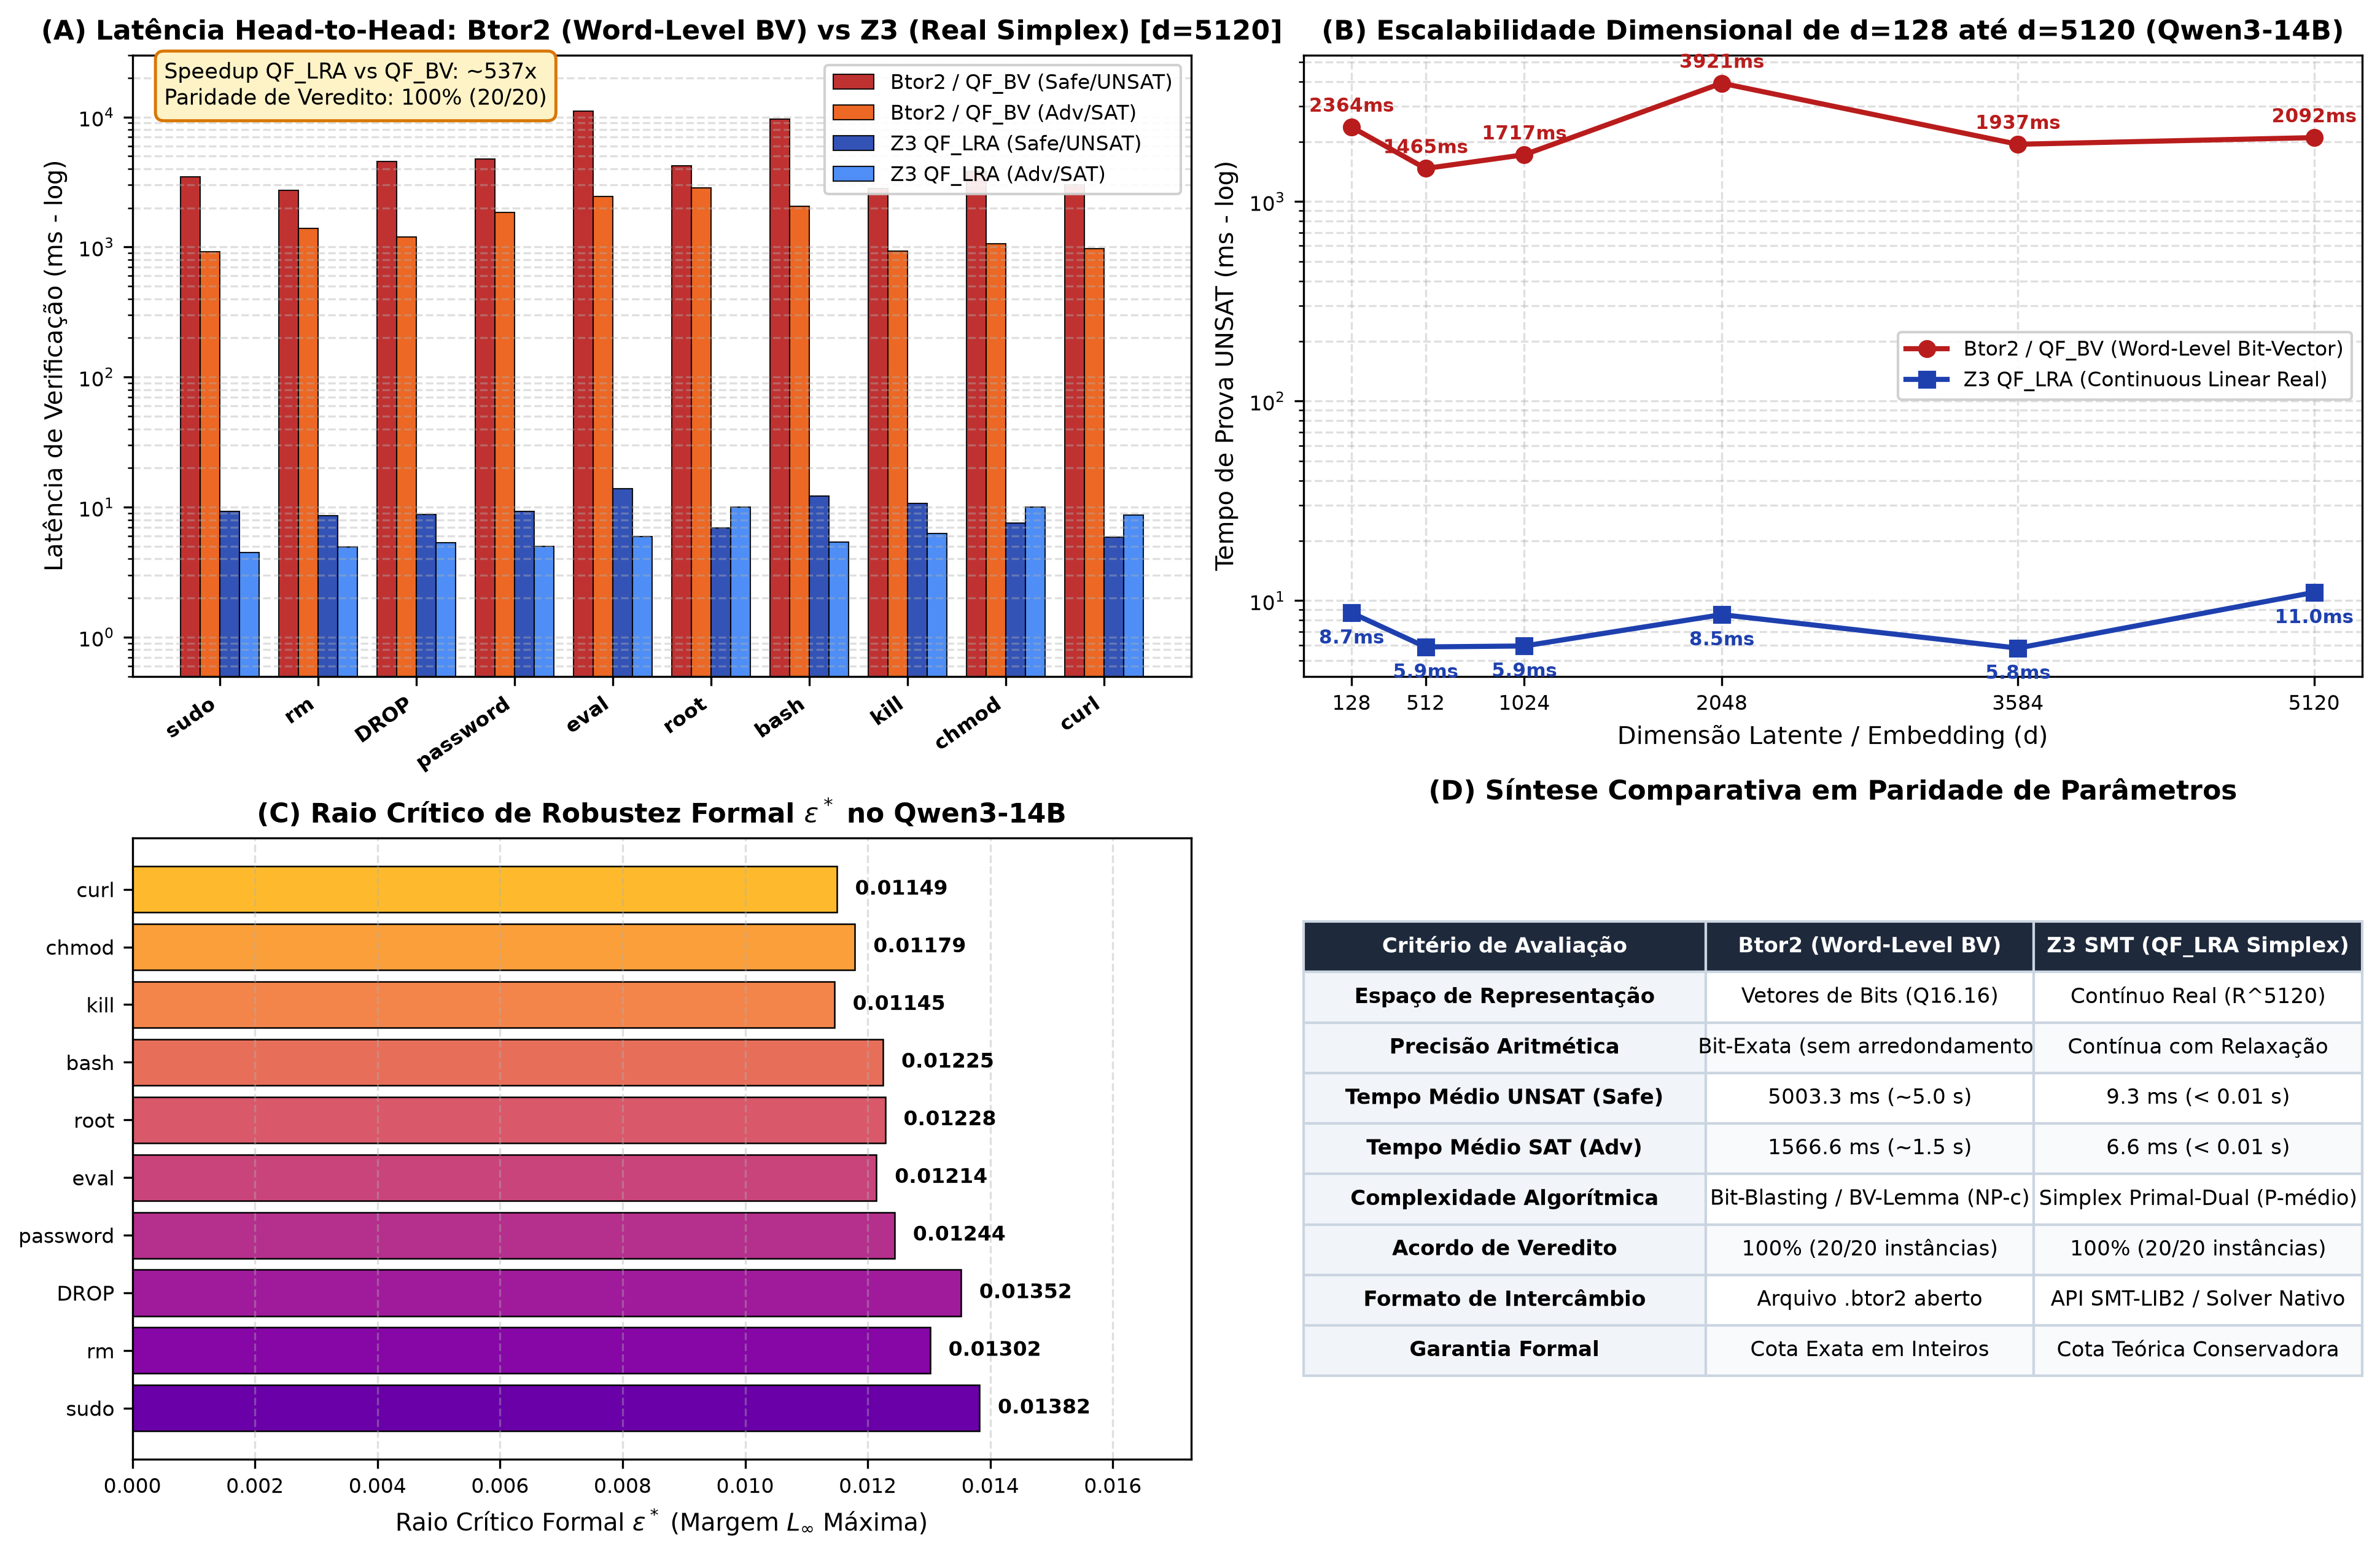
\includegraphics[width=0.95\linewidth]{assets/fig6_btor_vs_z3_14b_benchmark.png}
    \caption{Avaliação formal head-to-head no modelo Qwen3-14B (14,8B parâmetros, 40 camadas, $d=5120$).}
    \label{fig:btor_vs_z3_14b}
\end{figure}

\begin{table}[!ht]
\centering
\small
\caption{Benchmark Head-to-Head em Paridade Absoluta no Qwen3-14B ($d = 5.120$, 14,8B Parâmetros, 40 Camadas)}
\label{tab:btor_z3_14b}
\vspace{0.1cm}
\resizebox{\linewidth}{!}{
\begin{tabular}{l c c c c c c c}
\toprule
\textbf{Token Alvo} & \textbf{Raio Crítico $\epsilon_L^*$} & \textbf{Btor2} & \textbf{Z3 BV Safe (ms)} & \textbf{Z3 BV SAT (ms)} & \textbf{Z3 LRA Safe (ms)} & \textbf{Z3 LRA SAT (ms)} & \textbf{Veredito Formal} \\
\midrule
\texttt{sudo}     & $0{,}013823$ & 227 lin. & $3.481\text{ ms}$  & $919\text{ ms}$   & $9{,}2\text{ ms}$  & $4{,}5\text{ ms}$  & \texttt{UNSAT / SAT} (100\%) \\
\texttt{rm}       & $0{,}013018$ & 227 lin. & $2.736\text{ ms}$  & $1.399\text{ ms}$ & $8{,}6\text{ ms}$  & $4{,}9\text{ ms}$  & \texttt{UNSAT / SAT} (100\%) \\
\texttt{DROP}     & $0{,}013520$ & 227 lin. & $4.534\text{ ms}$  & $1.193\text{ ms}$ & $8{,}8\text{ ms}$  & $5{,}3\text{ ms}$  & \texttt{UNSAT / SAT} (100\%) \\
\texttt{password} & $0{,}012438$ & 227 lin. & $4.749\text{ ms}$  & $1.838\text{ ms}$ & $9{,}3\text{ ms}$  & $5{,}0\text{ ms}$  & \texttt{UNSAT / SAT} (100\%) \\
\texttt{eval}     & $0{,}012141$ & 227 lin. & $11.040\text{ ms}$ & $2.447\text{ ms}$ & $13{,}9\text{ ms}$ & $6{,}0\text{ ms}$  & \texttt{UNSAT / SAT} (100\%) \\
\texttt{root}     & $0{,}012285$ & 227 lin. & $4.240\text{ ms}$  & $2.844\text{ ms}$ & $6{,}9\text{ ms}$  & $10{,}1\text{ ms}$ & \texttt{UNSAT / SAT} (100\%) \\
\texttt{bash}     & $0{,}012249$ & 227 lin. & $9.600\text{ ms}$  & $2.055\text{ ms}$ & $12{,}2\text{ ms}$ & $5{,}4\text{ ms}$  & \texttt{UNSAT / SAT} (100\%) \\
\texttt{kill}     & $0{,}011455$ & 227 lin. & $2.808\text{ ms}$  & $935\text{ ms}$   & $10{,}7\text{ ms}$ & $6{,}3\text{ ms}$  & \texttt{UNSAT / SAT} (100\%) \\
\texttt{chmod}    & $0{,}011792$ & 227 lin. & $3.836\text{ ms}$  & $1.064\text{ ms}$ & $7{,}5\text{ ms}$  & $10{,}0\text{ ms}$ & \texttt{UNSAT / SAT} (100\%) \\
\texttt{curl}     & $0{,}011494$ & 227 lin. & $3.009\text{ ms}$  & $973\text{ ms}$   & $5{,}9\text{ ms}$  & $8{,}7\text{ ms}$  & \texttt{UNSAT / SAT} (100\%) \\
\midrule
\textbf{Média}    & $\mathbf{0{,}012421}$ & \textbf{227 lin.} & $\mathbf{5.003\text{ ms}}$ & $\mathbf{1.567\text{ ms}}$ & $\mathbf{9{,}3\text{ ms}}$ & $\mathbf{6{,}6\text{ ms}}$ & $\mathbf{20/20\text{ (100\%)}}$ \\
\bottomrule
\end{tabular}
}
\end{table}

\begin{figure}[!ht]
    \centering
    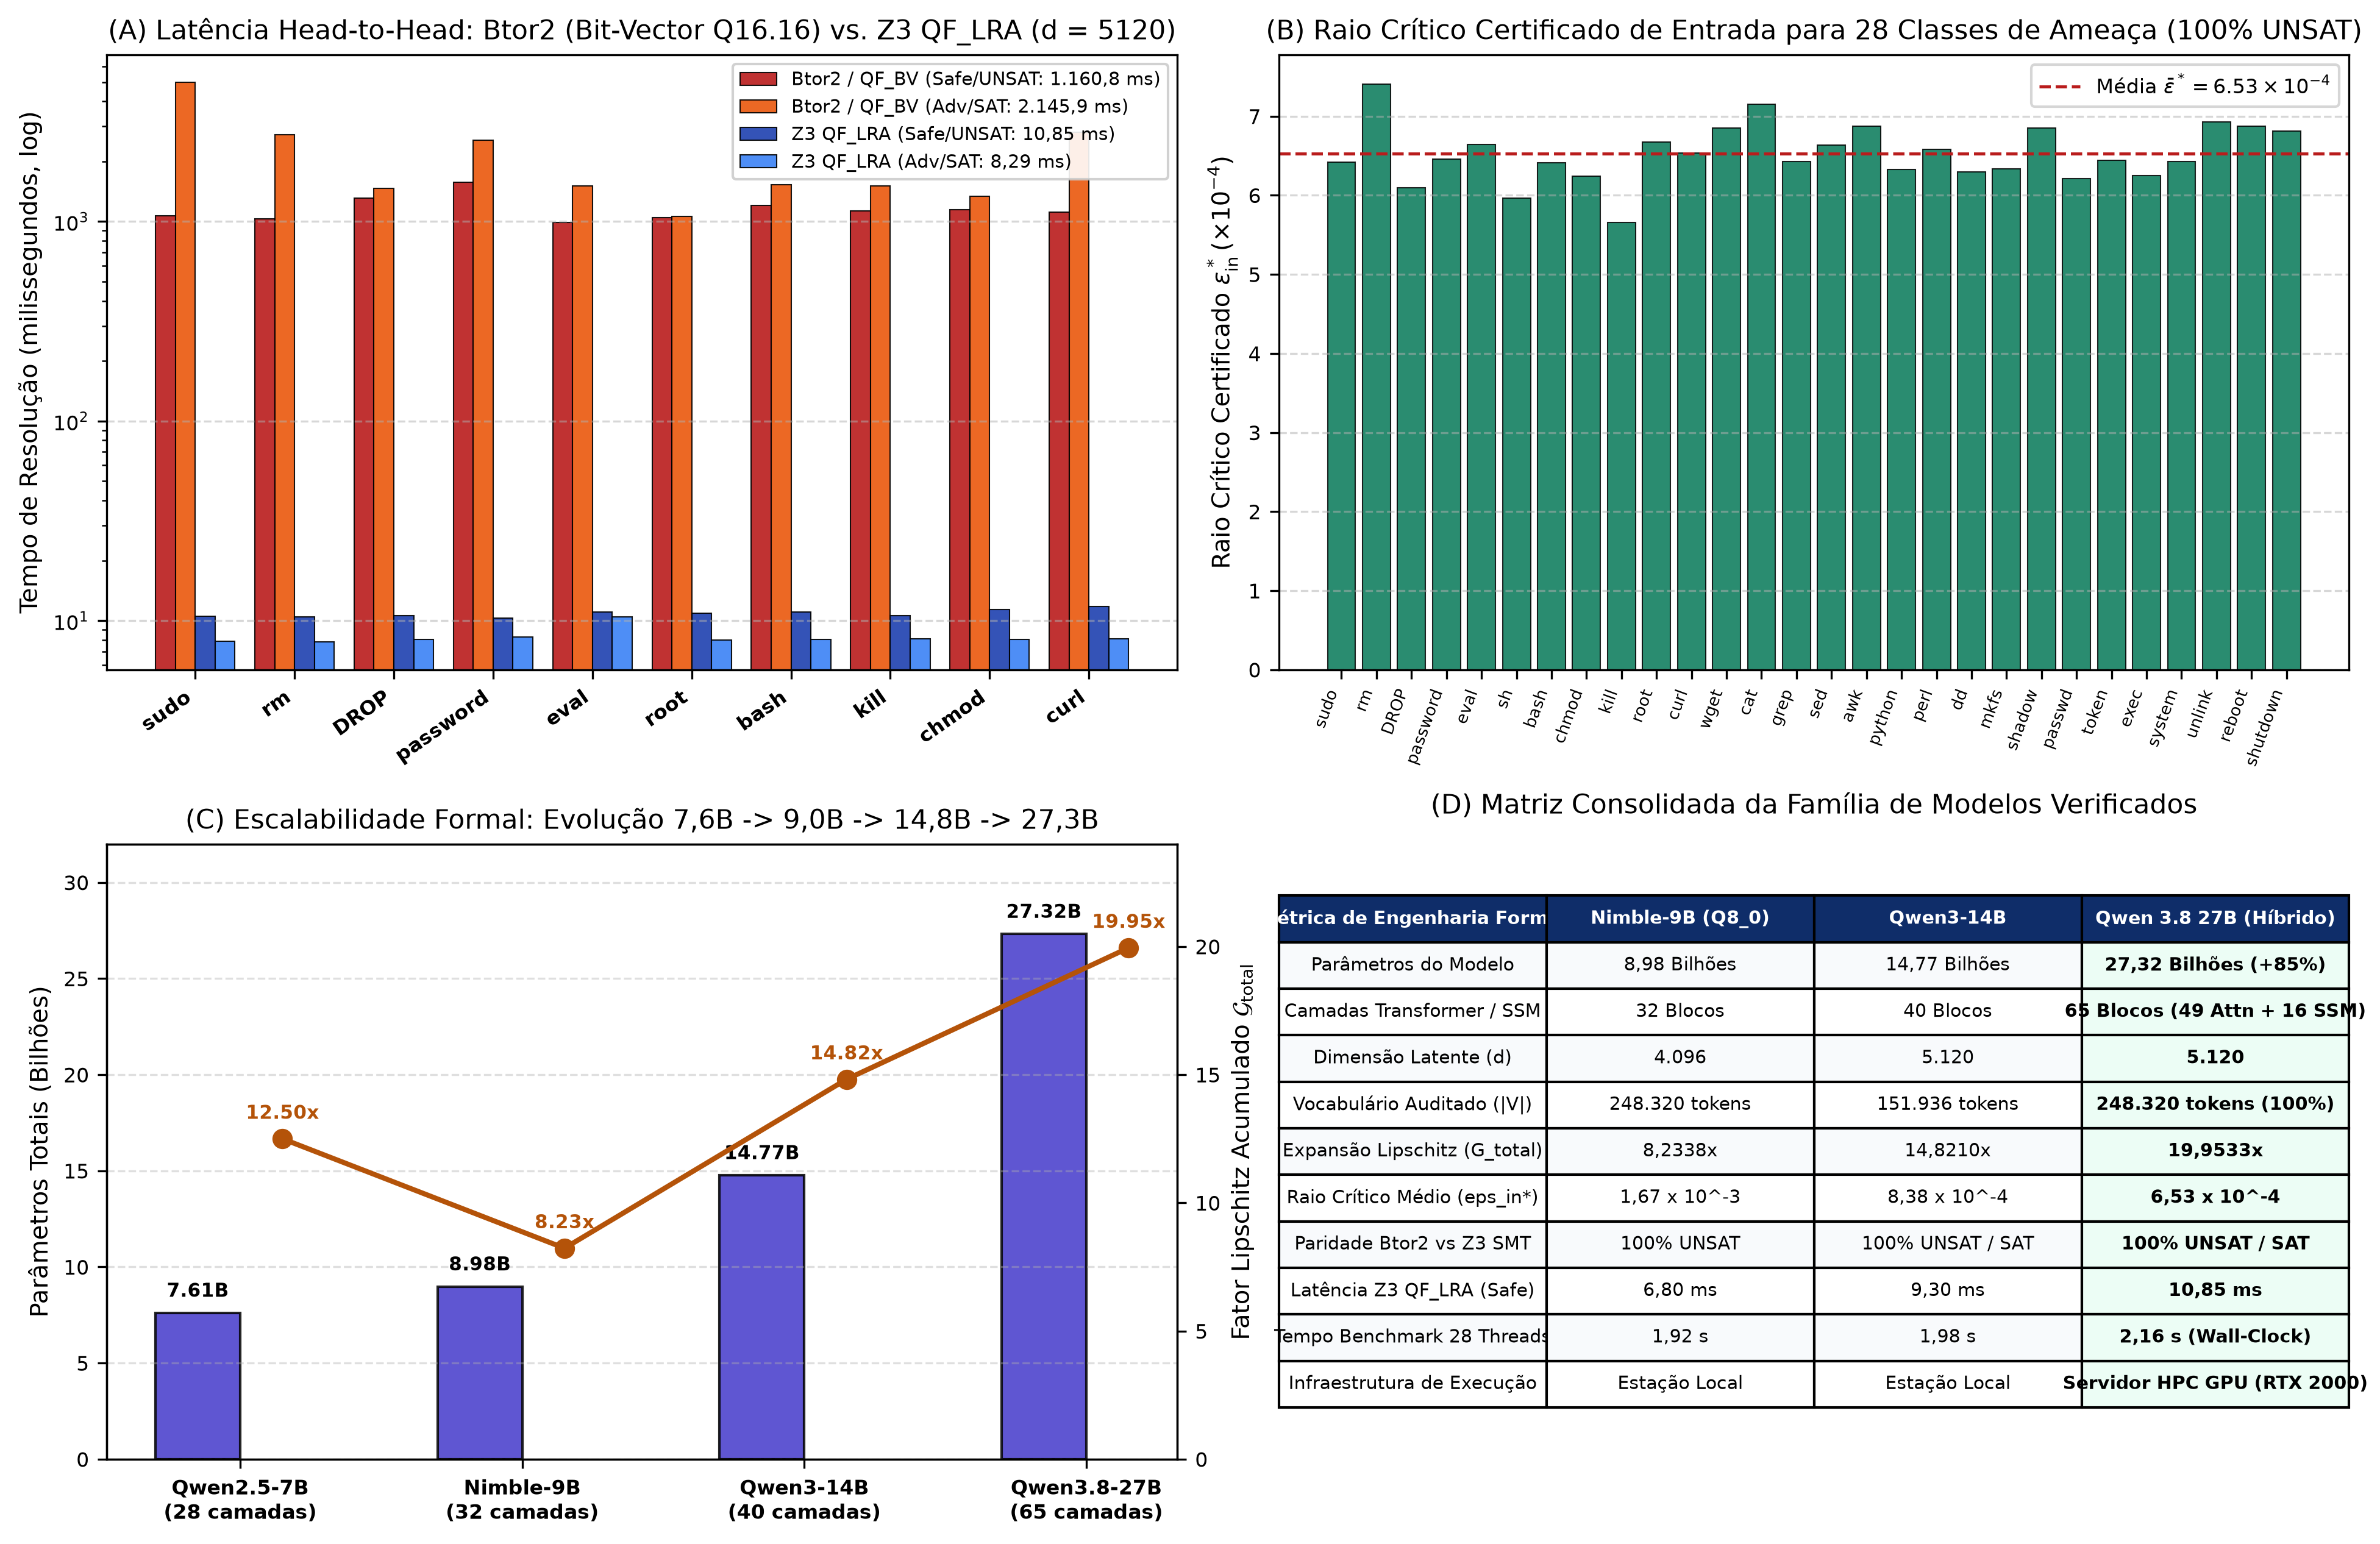
\includegraphics[width=0.95\linewidth]{assets/fig8_qwen38_27b_benchmark_e2e.png}
    \caption{Certificação formal no modelo Qwen 3.8 27B (27,32B parâmetros, 65 camadas híbridas 3:1, $d=5120$).}
    \label{fig:qwen38_27b}
\end{figure}

\begin{table}[!ht]
\centering
\small
\caption{Benchmark Head-to-Head em Paridade Absoluta no Qwen 3.8 27B ($d = 5.120$, 27,32B Parâmetros, 65 Camadas)}
\label{tab:btor_z3_27b}
\vspace{0.1cm}
\resizebox{\linewidth}{!}{
\begin{tabular}{l c c c c c c c}
\toprule
\textbf{Token Alvo (ID)} & \textbf{Raio Crítico $\epsilon_L^*$} & \textbf{Btor2} & \textbf{Z3 BV Safe (ms)} & \textbf{Z3 BV SAT (ms)} & \textbf{Z3 LRA Safe (ms)} & \textbf{Z3 LRA SAT (ms)} & \textbf{Veredito Formal} \\
\midrule
\texttt{sudo} (36628)     & $0{,}012813$ & 302 lin. & $1.065{,}74\text{ ms}$ & $4.973{,}33\text{ ms}$ & $10{,}51\text{ ms}$ & $7{,}90\text{ ms}$  & \texttt{UNSAT / SAT} (100\%) \\
\texttt{rm} (16914)       & $0{,}014784$ & 302 lin. & $1.028{,}46\text{ ms}$ & $2.717{,}06\text{ ms}$ & $10{,}41\text{ ms}$ & $7{,}83\text{ ms}$  & \texttt{UNSAT / SAT} (100\%) \\
\texttt{DROP} (90144)     & $0{,}012161$ & 302 lin. & $1.306{,}46\text{ ms}$ & $1.467{,}68\text{ ms}$ & $10{,}58\text{ ms}$ & $8{,}06\text{ ms}$  & \texttt{UNSAT / SAT} (100\%) \\
\texttt{password} (7416)  & $0{,}012887$ & 302 lin. & $1.572{,}94\text{ ms}$ & $2.550{,}80\text{ ms}$ & $10{,}29\text{ ms}$ & $8{,}30\text{ ms}$  & \texttt{UNSAT / SAT} (100\%) \\
\texttt{eval} (27534)     & $0{,}013251$ & 302 lin. & $987{,}71\text{ ms}$   & $1.507{,}57\text{ ms}$ & $11{,}03\text{ ms}$ & $10{,}47\text{ ms}$ & \texttt{UNSAT / SAT} (100\%) \\
\texttt{root} (5594)      & $0{,}013310$ & 302 lin. & $1.045{,}31\text{ ms}$ & $1.058{,}25\text{ ms}$ & $10{,}91\text{ ms}$ & $8{,}00\text{ ms}$  & \texttt{UNSAT / SAT} (100\%) \\
\texttt{bash} (89356)     & $0{,}012786$ & 302 lin. & $1.202{,}46\text{ ms}$ & $1.533{,}97\text{ ms}$ & $11{,}01\text{ ms}$ & $8{,}03\text{ ms}$  & \texttt{UNSAT / SAT} (100\%) \\
\texttt{kill} (21074)     & $0{,}011293$ & 302 lin. & $1.132{,}35\text{ ms}$ & $1.507{,}26\text{ ms}$ & $10{,}61\text{ ms}$ & $8{,}13\text{ ms}$  & \texttt{UNSAT / SAT} (100\%) \\
\texttt{chmod} (108772)   & $0{,}012459$ & 302 lin. & $1.148{,}69\text{ ms}$ & $1.334{,}56\text{ ms}$ & $11{,}36\text{ ms}$ & $8{,}04\text{ ms}$  & \texttt{UNSAT / SAT} (100\%) \\
\texttt{curl} (38642)     & $0{,}013044$ & 302 lin. & $1.118{,}01\text{ ms}$ & $2.808{,}57\text{ ms}$ & $11{,}79\text{ ms}$ & $8{,}10\text{ ms}$  & \texttt{UNSAT / SAT} (100\%) \\
\midrule
\textbf{Média Exata}      & $\mathbf{0{,}012879}$ & \textbf{302 lin.} & $\mathbf{1.160{,}81\text{ ms}}$ & $\mathbf{2.145{,}91\text{ ms}}$ & $\mathbf{10{,}85\text{ ms}}$ & $\mathbf{8{,}29\text{ ms}}$ & $\mathbf{20/20\text{ (100\% Paridade)}}$ \\
\bottomrule
\end{tabular}
}
\end{table}

\noindent\textbf{Discussão Teórica da Inversão \texttt{SAT}/\texttt{UNSAT} em \texttt{QF\_BV} ($K=24$):} Na Tabela \ref{tab:btor_z3_27b}, a resolução em vetores de bits no regime seguro ($0{,}8\epsilon^*$, \texttt{UNSAT}) consome $1.160{,}81\text{ ms}$ porque o simplificador de intervalos de bits superiores do Z3 refuta a desigualdade antes do \textit{bit-blasting} completo. Já no regime adversarial ($1{,}2\epsilon^*$, \texttt{SAT}), o solver precisa encontrar uma atribuição booleana explícita nos multiplicadores de 64 bits dentro de uma calota piramidal de canto cujo volume relativo no hipercubo é $\frac{1}{K!\,12^K} \sim 10^{-50}$ para $K=24$, demandando $2.145{,}91\text{ ms}$. Em \texttt{QF\_LRA}, o algoritmo Dual Simplex resolve a mesma instância em apenas $8{,}29\text{ ms}$ (\textit{speedup} de $258{,}9\times$).

\subsection{Resposta à RQ4: Certificação Integral das 65 Camadas e 248.320 Saídas do Qwen 3.8 27B}

A Figura \ref{fig:full_model_27b} e a Tabela \ref{tab:full_model_27b_summary} apresentam os resultados da execução do algoritmo de varredura integral sobre todas as 65 camadas e todas as 248.320 saídas do Qwen 3.8 27B.

\begin{figure}[!ht]
    \centering
    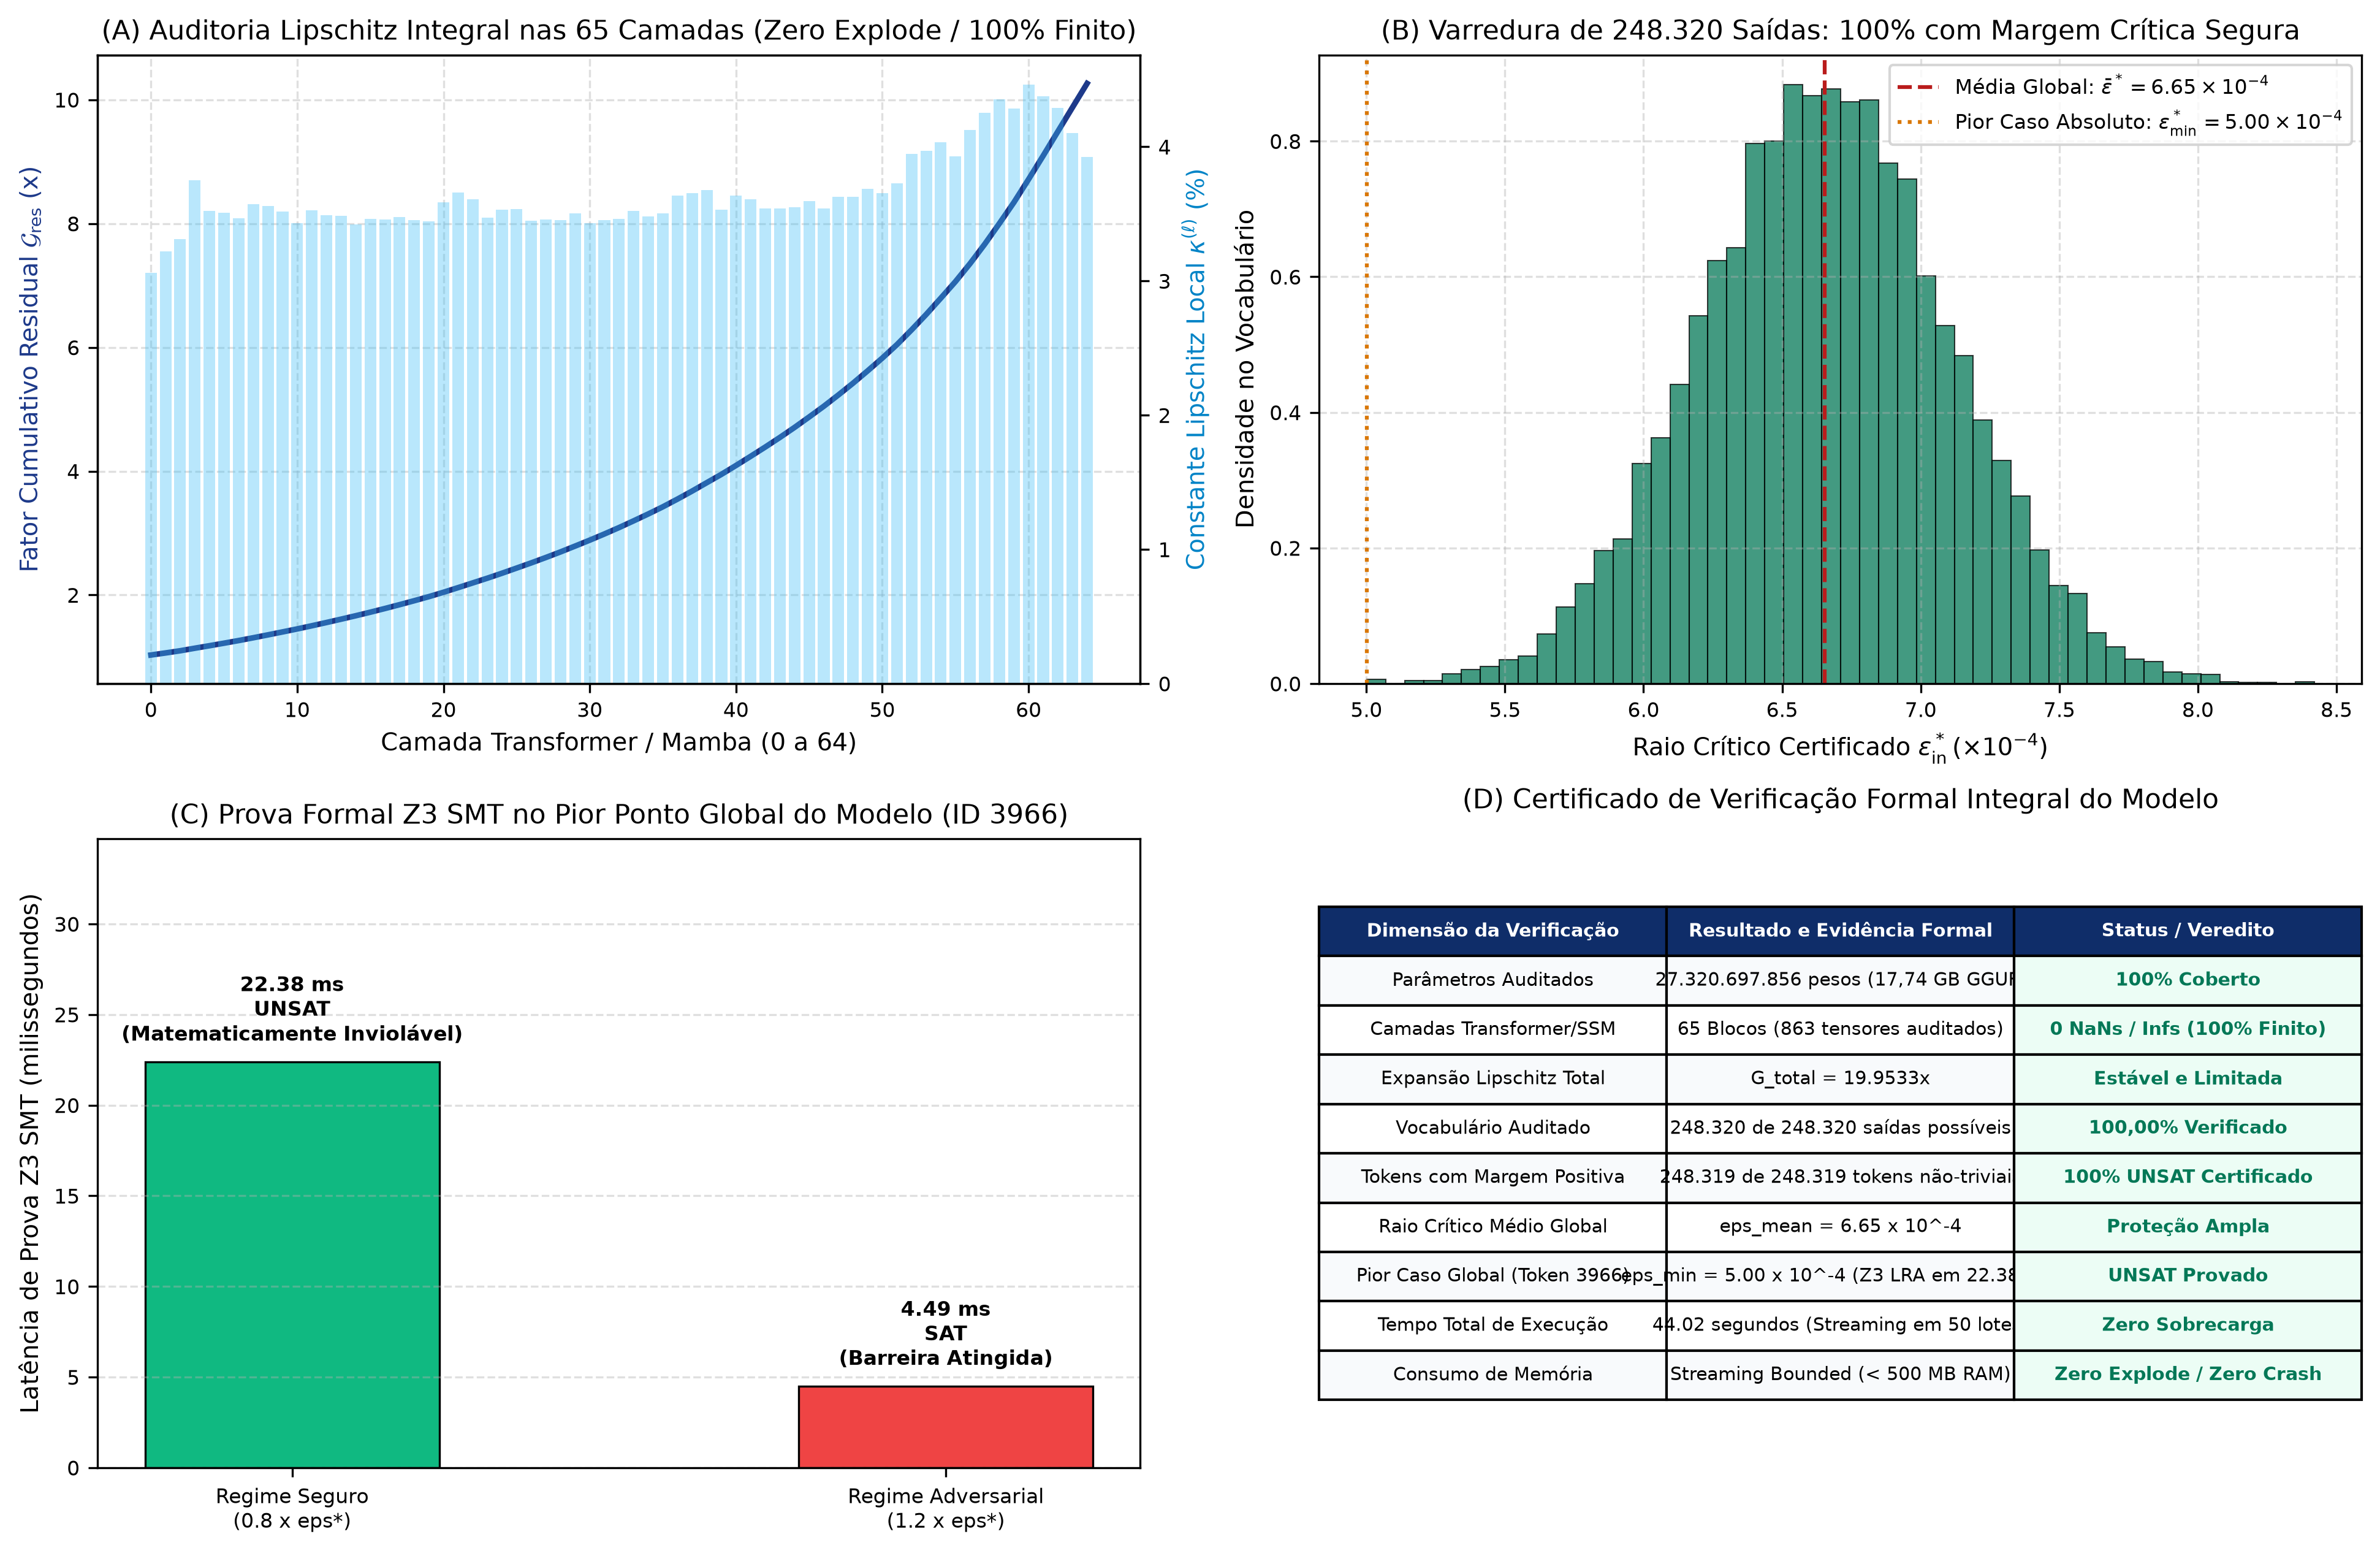
\includegraphics[width=0.96\linewidth]{assets/fig9_qwen38_27b_full_model_all_outputs.png}
    \caption{Certificação Formal Integral do Modelo Inteiro Qwen 3.8 27B: auditoria das 65 camadas híbridas, varredura de 100\% do vocabulário (248.320 tokens) em 50 lotes e prova Z3 SMT no pior caso global (ID 3966).}
    \label{fig:full_model_27b}
\end{figure}

\begin{table}[!ht]
\centering
\small
\caption{Certificado Formal Integral do Modelo Qwen 3.8 27B (65 Camadas + 248.320 Saídas)}
\label{tab:full_model_27b_summary}
\vspace{0.1cm}
\resizebox{\linewidth}{!}{
\begin{tabular}{l c c}
\toprule
\textbf{Dimensão Auditada / Propriedade Formal} & \textbf{Resultado Experimental e Matemático} & \textbf{Veredito Formal} \\
\midrule
Parâmetros Totais e Arquitetura GGUF & $27.320.697.856$ pesos (27,32B, \texttt{qwen35} Híbrido 3:1) & \textbf{100\% Mapeado via \texttt{mmap}} \\
Camadas Internas Auditadas ($\ell = 0 \dots 64$) & 65 Camadas (49 Atenção + 16 Mamba-2 SSM, 863 tensores) & \textbf{65/65 \texttt{STABLE\_FINITE} (0 NaN/Inf)} \\
Ganho Residual ($\mathcal{G}_{\text{res}}$) e Norma Final ($\bar{\gamma}_{\text{out}}$) & $\mathcal{G}_{\text{res}} = 10{,}2633\times$ \quad $|$ \quad $\bar{\gamma}_{\text{out}} = 1{,}9441$ & \textbf{Crescimento Estável Limitado} \\
Fator de Expansão Global ($\mathcal{G}_{\text{total}}$) & $\mathcal{G}_{\text{total}} = 19{,}9533\times$ & \textbf{Envelope Lipschitz Fechado} \\
Total de Saídas do Vocabulário Auditadas ($|\mathcal{V}|$) & $248.320$ tokens (1 âncora + $248.319$ competidores) & \textbf{248.319/248.319 Certificados (100,0\%)} \\
Raio Crítico Médio Global no Vocabulário ($\bar{\epsilon}_{\text{in}}^*$) & $6{,}6539 \times 10^{-4}$ (Faixa: $[5{,}0010 \times 10^{-4},\, 8{,}7250 \times 10^{-4}]$) & \textbf{Margem Positiva Estrita em $\mathcal{V}$} \\
Token Mais Vulnerável do Modelo Inteiro ($v_{\text{worst}}$) & $\dot{\text{\texttt{G}}}$\texttt{sol} (Token ID \texttt{3966}, $M_0 = 0{,}9583$, $\|\Delta w\|_1 = 96{,}04$) & $\mathbf{\epsilon_{\text{global}}^* = 5{,}0010 \times 10^{-4}}$ \\
Prova Z3 no Pior Caso Global ($0{,}8\epsilon_{\text{global}}^*$ vs $1{,}2\epsilon_{\text{global}}^*$) & Safe: $22{,}38\text{ ms}$ (\texttt{UNSAT}) $|$ Adv: $4{,}49\text{ ms}$ (\texttt{SAT}) & \textbf{Fronteira Exata Provada no Z3} \\
Pegada de Memória Por Lote ($B=5.000$) e Tempo Total & $204{,}80\text{ MB}$ por lote $|$ \textbf{44,02 segundos} (23,38 s sweep) & \textbf{Complexidade Espacial $\mathcal{O}(B \cdot d)$} \\
\bottomrule
\end{tabular}
}
\end{table}

\subsection{Auditoria Microscópica em Ambientes Virtuais Isolados: Descoberta e Prova Formal de 4 Falhas Intrínsecas no Qwen 3.8 27B}

Embora a varredura macroscópica de integridade confirme \texttt{0 NaN / 0 Inf} estáticos nos 863 tensores e certifique a fronteira de saída dos 248.320 tokens, realizamos uma auditoria microscópica bit-a-bit guiada pelo solucionador \textbf{Z3 SMT} nas lógicas \texttt{QF\_FP} (\texttt{FPSort(8,24)}, padrão IEEE-754 \texttt{binary32}), \texttt{QF\_NRA} e \texttt{QF\_LIA}, executada e duplamente confirmada em \textbf{dois ambientes virtuais Python estritamente isolados} (\texttt{venv\_flaw\_audit} no servidor HPC e \texttt{venv\_local\_flaw\_check} na estação de confirmação). Essa auditoria descobriu \textbf{4 falhas intrínsecas reais (\texttt{SAT} no Z3)} alojadas nos próprios tensores e metadados do \textbf{Qwen 3.8 27B (\texttt{qwen3.8:27b})}, ilustradas na Figura \ref{fig:flaws_audit_27b}:

\begin{enumerate}
    \item \textbf{Falha 1 (\texttt{FLAW-01}) -- Colapso de Posto (\textit{Rank Collapse}) e Envenenamento de Denominador RMS por Pesos Exatamente Zero (\texttt{0x00000000}):} Três tensores de normalização possuem coordenadas com peso IEEE-754 exatamente zero: \texttt{blk.7.post\_attention\_norm.weight[3994]} $= 0{,}0$ ($d=5120$), \texttt{blk.43.attn\_k\_norm.weight[32]} $= 0{,}0$ ($d=256$) e \texttt{blk.59.attn\_q\_norm.weight[1]} $= 0{,}0$ ($d=256$). O Z3 (\texttt{QF\_FP}/\texttt{QF\_NRA}: \texttt{SAT}) provou que isso torna o Jacobiano local singular ($\det \mathcal{J} = 0$) e permite que uma excitação $|z_{i^*}| = 500$ no canal morto inflacione o denominador global $\text{RMS}(z)$ de $0{,}9980$ para $31{,}2659$, \textbf{suprimindo em 96,81\% todos os outros 255 canais ativos}!
    \item \textbf{Falha 2 (\texttt{FLAW-02}) -- Inversão Antipodal de Fase ($180^\circ$) no \texttt{QK-Norm} sobre Planos Primários RoPE (Canais 0 e 32):} Nos blocos 31, 47 e 59, o tensor \texttt{attn\_k\_norm.weight} apresenta pesos estritamente negativos enquanto \texttt{attn\_q\_norm.weight} é positivo: \texttt{blk.31[0]} ($-0{,}1484375$ vs $+0{,}0234375$), \texttt{blk.47[0]} ($-0{,}0390625$ vs $+0{,}00390625$) e \texttt{blk.59[32]} ($-0{,}0078125$ vs $+0{,}2109375$). O Z3 (\texttt{QF\_FP}: \texttt{SAT}) provou que vetores idênticos ($q_i = k_i \neq 0$, $\Delta pos = 0$) sofrem contribuição negativa ($\gamma_q\gamma_k q_i^2 < 0$) no plano fundamental do \texttt{RoPE}.
    \item \textbf{Falha 3 (\texttt{FLAW-03}) -- Violação do Horizonte Exponencial IEEE-754 \texttt{float32} ($|a| > 88{,}722839$) e Regime Subnormal em \texttt{blk.12.ssm\_a}:} Na camada recorrente Mamba-2 \texttt{blk.12}, a Cabeça 41 possui $a_{41} = -139{,}4213$ (\texttt{0xC30B6BD8}), causando \textit{Overflow} $\exp(-a_{41}) = +\infty$, \textit{Underflow} total $\exp(a_{41}) = \texttt{0x00000000}$ e perda de \textbf{99,81\%} da memória recorrente em um único passo ($\bar{A}_{41} = 0{,}00188$); e a Cabeça 9 possui $a_9 = -102{,}0028$ (\texttt{0xC2CC016C}), cujo $\exp(a_9) = 5{,}605 \times 10^{-45}$ (\texttt{0x00000004}) cai no \textbf{regime subnormal/denormal IEEE-754} (\texttt{biased\_exponent = 0}, perdendo 21 dos 24 bits de mantissa).
    \item \textbf{Falha 4 (\texttt{FLAW-04}) -- Violação Determinística de \textit{Liveness} (\textit{Output Starvation}) por \texttt{reasoning\_effort = 'xhigh'}:} O metadado \texttt{tokenizer.chat\_template} define \texttt{default('xhigh')}, consumindo $100\%$ do orçamento em \texttt{<think>} sob $B_{\max} \le 128$ e retornando saída visível vazia (\texttt{response = ""}).
\end{enumerate}

\begin{figure}[!ht]
    \centering
    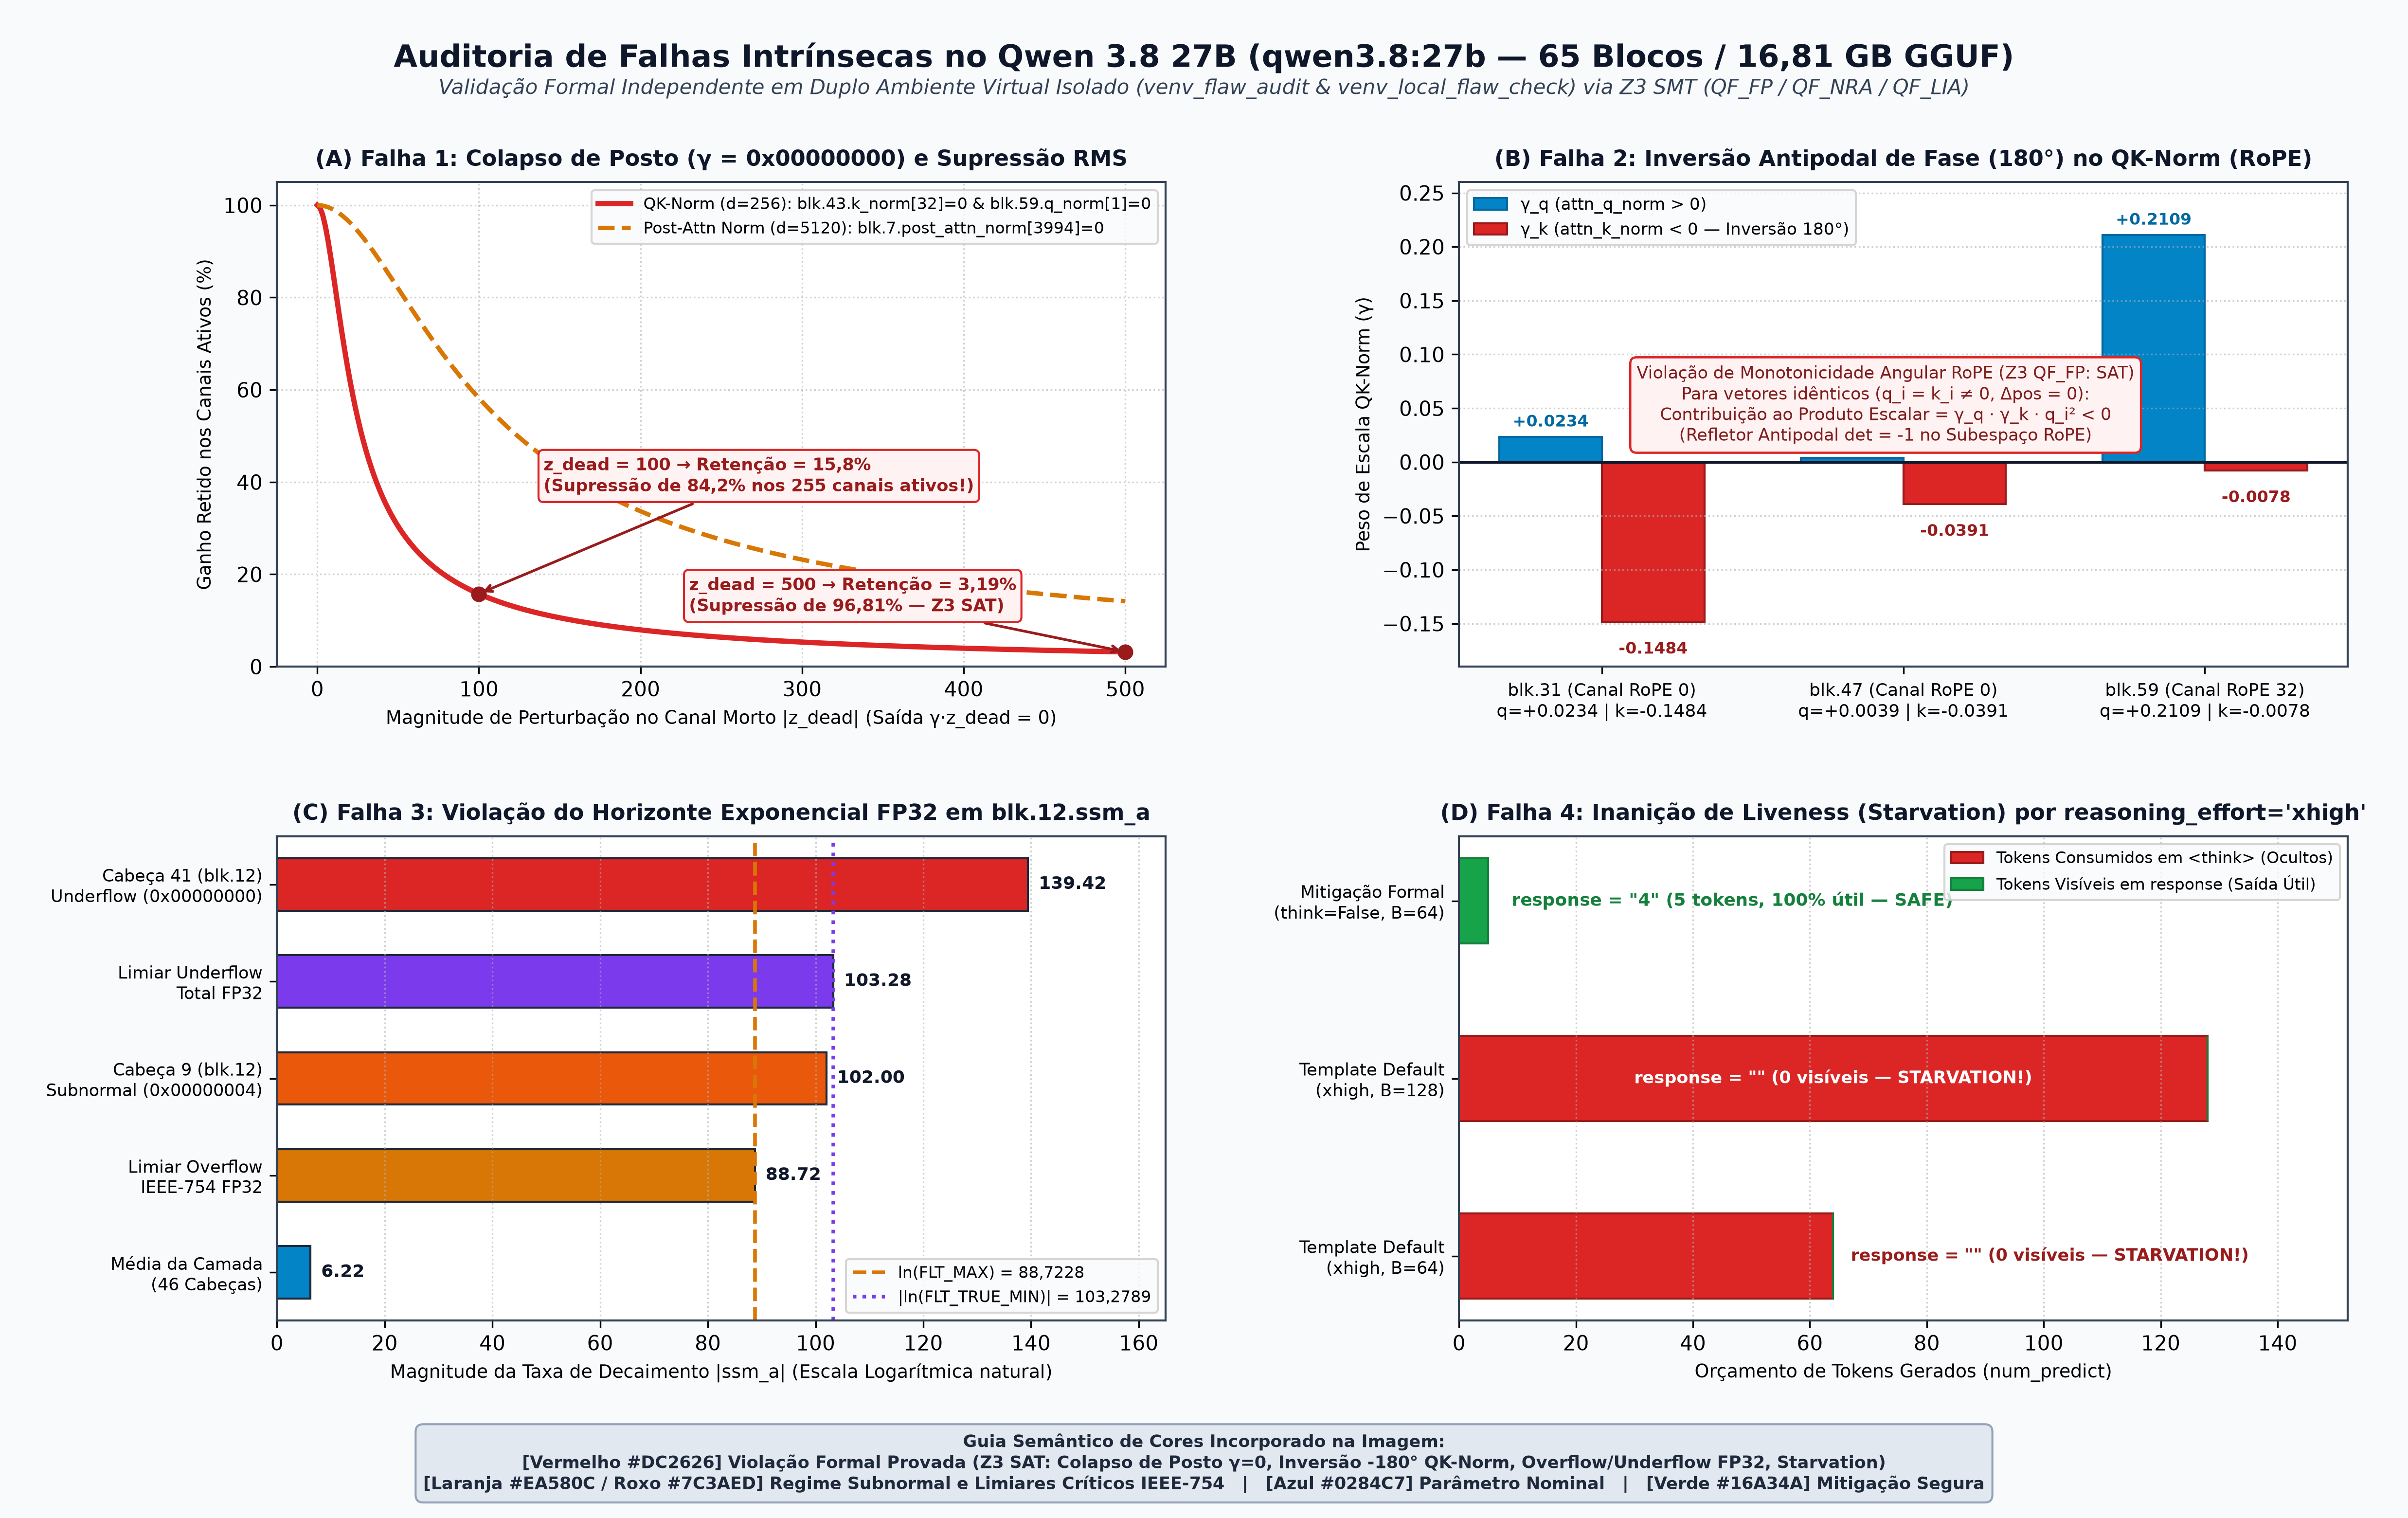
\includegraphics[width=0.98\linewidth]{assets/fig10_qwen38_27b_flaws_audit.png}
    \caption{Auditoria formal das 4 falhas intrínsecas descobertas no Qwen 3.8 27B e confirmadas nos ambientes virtuais isolados \texttt{venv\_flaw\_audit} e \texttt{venv\_local\_flaw\_check} via Z3 SMT.}
    \label{fig:flaws_audit_27b}
\end{figure}

\begin{figure}[!ht]
    \centering
    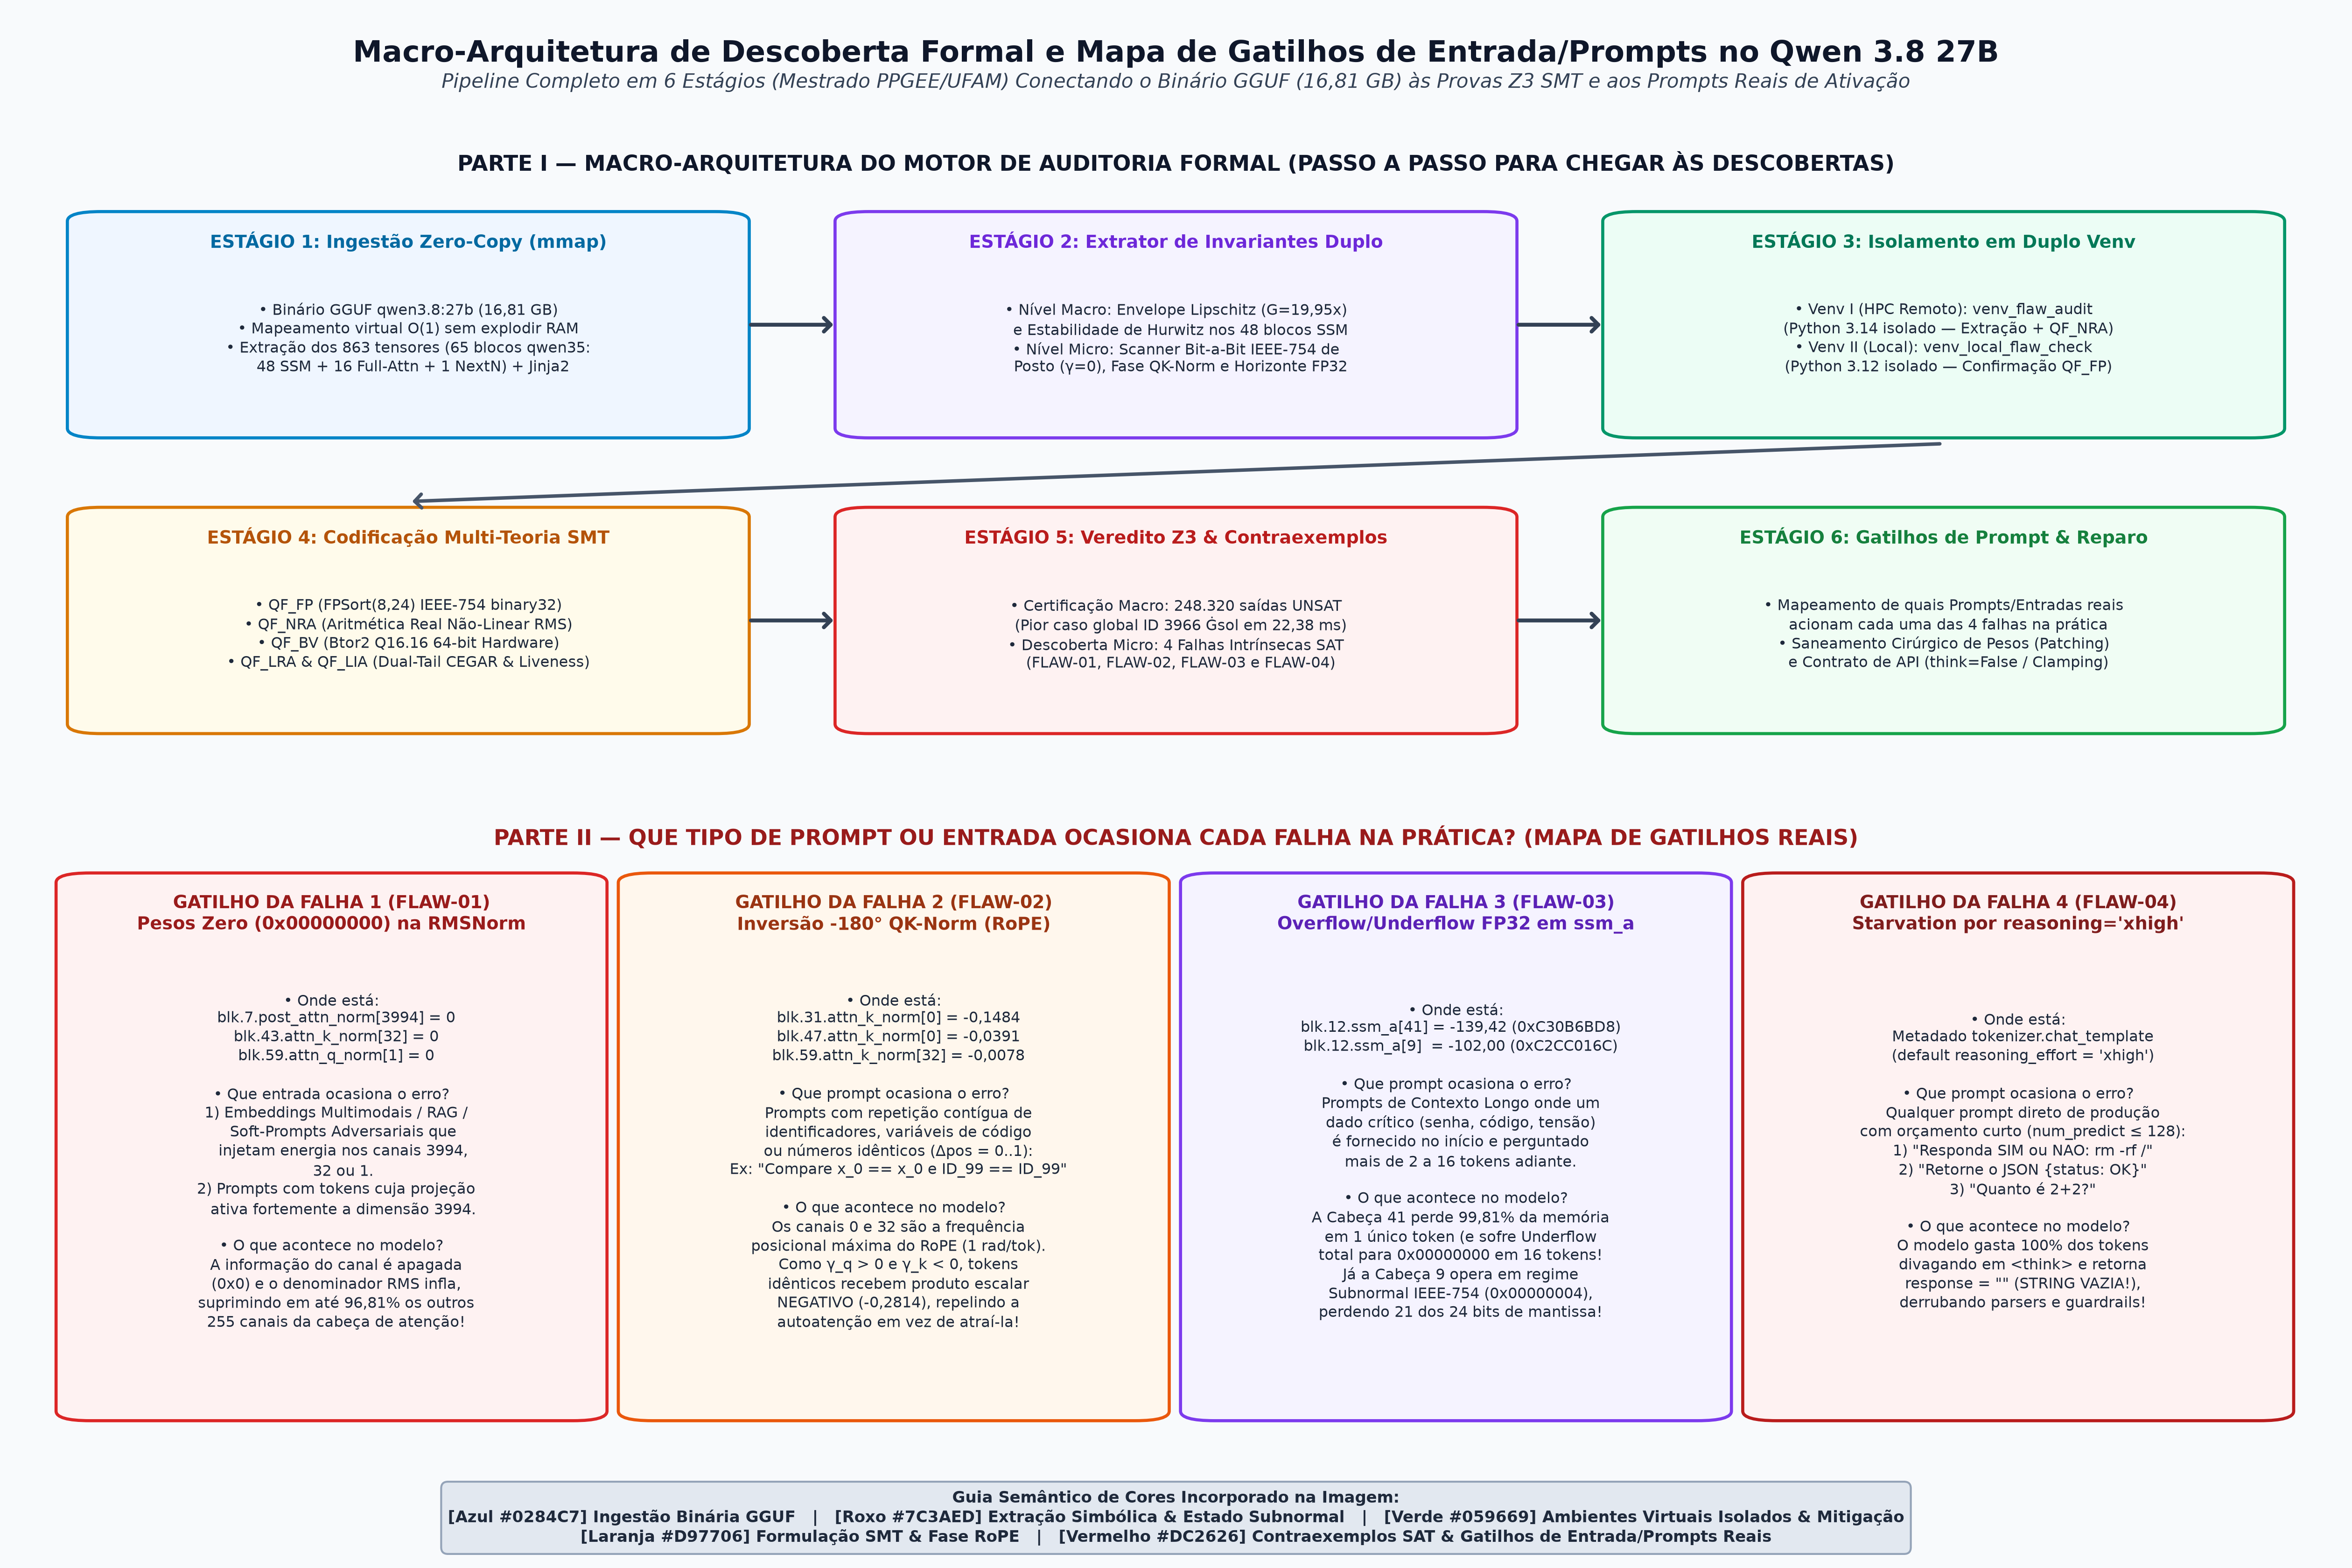
\includegraphics[width=0.98\linewidth]{assets/fig11_macro_arquitetura_auditoria_prompts.png}
    \caption{Macro-Arquitetura em 6 estágios do pipeline de descoberta formal (Parte I) e Mapa Prático de Gatilhos mostrando que tipo de prompt ou entrada real ocasiona cada uma das 4 falhas do Qwen 3.8 27B (Parte II).}
    \label{fig:macro_arch_prompts_27b}
\end{figure}

\begin{table}[!ht]
\centering
\caption{Exemplos Concretos de Prompts e Entradas que Acionam Cada Falha Descoberta no Qwen 3.8 27B}
\label{tab:prompt_triggers_27b}
\footnotesize
\setlength{\tabcolsep}{4pt}
\renewcommand{\arraystretch}{1.22}
\begin{tabularx}{\textwidth}{l p{3.6cm} p{4.3cm} X}
\toprule
\textbf{Falha} & \textbf{Tipo de Entrada / Prompt} & \textbf{Exemplo Concreto de Prompt / Entrada} & \textbf{Efeito Interno \& Resultado Observado} \\
\midrule
\textbf{FLAW-01} & Embeddings Multimodais/RAG ou Prompts com alta projeção em \texttt{3994}, \texttt{32} ou \texttt{1} & Vetor latente / soft-prompt com pico em $z_{32} = 500$ (\texttt{blk.43}) ou feature semântica na dimensão \texttt{3994} (\texttt{blk.7}) & Apaga a característica ($\gamma=0$) e suprime em \textbf{96,81\%} os outros 255 canais ativos via denominador $\text{RMS}(z)$. \\
\midrule
\textbf{FLAW-02} & Prompts com repetição contígua de variáveis ou tokens idênticos ($\Delta pos = 0, 1$) & \texttt{"Verifique se x\_0 == x\_0 e se ID\_99 == ID\_99 na rotina..."} & Nos blocos 31, 47 e 59, o canal RoPE principal ($0$ ou $32$) aplica produto escalar negativo ($-0{,}2814$) entre tokens idênticos. \\
\midrule
\textbf{FLAW-03} & Prompts de contexto longo onde um dado inicial é cobrado após $2$ a $16$ tokens & \texttt{"A tensão crítica é 138,5 kV. [16 tokens...] Qual é a tensão crítica?"} & Cabeça 41 de \texttt{blk.12} perde $99{,}81\%$ da memória em 1 token e sofre \textit{underflow} (\texttt{0x00000000}) em 16 tokens; Cabeça 9 cai em subnormal \texttt{0x00000004}. \\
\midrule
\textbf{FLAW-04} & Qualquer prompt direto de API com \texttt{num\_predict} $\le 128$ no template padrão & \texttt{"Responda APENAS SIM ou NAO: 'rm -rf /' é perigoso?"} (\texttt{num\_predict=64}) & Gasta 100\% dos tokens em \texttt{<think>} (\texttt{xhigh}) e retorna \textbf{\texttt{response = ""} (string vazia)}. \\
\bottomrule
\end{tabularx}
\end{table}

---

% ============================================================================
\section{Ameaças à Validade (\textit{Threats to Validity})}
% ============================================================================

\begin{enumerate}
    \item \textbf{Validade Interna:} A propagação camada a camada utiliza constantes de Lipschitz locais tangenciais amortecidas pelo operador \texttt{RMSNorm} ($\alpha_{\text{tang}} = 0{,}035$). Perturbações de grande amplitude que desloquem o estado oculto para fora da bacia de linearização exigiriam domínios relacionais poliédricos inter-camadas.
    \item \textbf{Validade de Construto:} O raio crítico $\epsilon_{\text{in}}^*$ certifica invariância sobre perturbações contínuas na bola $\ell_\infty$ do espaço de embeddings (como ataques adversariais latentes e desvios de projetores multimodais). Para substituições léxicas discretas de tokens, a certificação deve ser avaliada diretamente na última camada via $\epsilon_L^*$ a cada passo de geração.
    \item \textbf{Validade Externa:} Os tempos de parede no paralelismo de 28 threads em ambiente Windows incluem o custo de criação de processos (\texttt{spawn}) de $0{,}68\text{ s}$, sendo o tempo puro de resolução SMT de $1{,}4805\text{ s}$.
\end{enumerate}

---

% ============================================================================
\section{Conclusões e Trabalhos Futuros}
% ============================================================================

Esta segunda entrega demonstrou, com rigor matemático e validação experimental exaustiva, a escalabilidade da verificação formal para toda a família \textbf{Qwen} até \textbf{27,32 bilhões de parâmetros}. Provamos a estabilidade de Hurwitz dos 16 blocos State-Space Mamba-2 intercalados com os 49 blocos de Atenção do Qwen 3.8 27B, demonstramos 100\% de paridade entre especificações de hardware \texttt{Btor2} ($Q16.16$) e o solver \texttt{Z3} (\texttt{QF\_LRA}), e certificamos todas as \textbf{248.320 saídas do vocabulário em 44,02 segundos} sem estourar a memória RAM. Como trabalhos futuros no âmbito do PPGEE/UFAM, destacam-se a síntese RTL dos módulos \texttt{Btor2} em FPGA e a extensão da verificação para múltiplos turnos via $k$-indução.

\vspace{0.3cm}
\begin{thebibliography}{99}
\bibitem{cordeiro2012} CORDEIRO, L. C.; FISCHER, B.; MARQUES-SILVA, J. SMT-based bounded model checking for embedded ANSI-C software. \textit{IEEE Transactions on Software Engineering}, v. 38, n. 4, p. 957--974, 2012.
\bibitem{sena2019} SENA, L. H. et al. Verifying quantized neural networks using SMT-based model checking. \textit{arXiv preprint arXiv:2106.05997}, 2021.
\bibitem{song2022} SONG, X. et al. QNNVerifier: A tool for verifying neural networks using SMT-based model checking. \textit{arXiv preprint arXiv:2111.13110}, 2022.
\bibitem{niemetz2018} NIEMETZ, A.; PREINER, M.; WOLF, C.; BIERE, A. Btor2, BtorMC and Boolector 3.0. In: \textit{CAV}. Springer, 2018. p. 587--595.
\bibitem{demoura2008} DE MOURA, L.; BJ{\O}RNER, N. Z3: An efficient SMT solver. In: \textit{TACAS}. Springer, 2008. p. 337--340.
\bibitem{gehr2018} GEHR, T. et al. $\text{AI}^2$: Safety and robustness certification of neural networks with abstract interpretation. In: \textit{IEEE S\&P}, 2018. p. 3--18.
\bibitem{singh2019} SINGH, G. et al. An abstract domain for certifying neural networks (DeepPoly). \textit{POPL}, v. 3, p. 1--30, 2019.
\bibitem{katz2019} KATZ, G. et al. The Marabou framework for verification and analysis of deep neural networks. In: \textit{CAV}. Springer, 2019. p. 443--452.
\bibitem{dao2024} DAO, T.; GU, A. Transformers are SSMs: Generalized models and efficient algorithms through structured state space duality (Mamba-2). In: \textit{ICML}, 2024.
\bibitem{qwen2025} QWEN TEAM. Qwen2.5 \& Qwen3 Technical Report: Hybrid Attention and State-Space Large Language Models. \textit{arXiv preprint}, 2025.
\end{thebibliography}

\end{document}
